\documentclass[12pt,american,english, pointlessnumbers, abstracton, headsepline]{scrreprt}

\renewcommand{\familydefault}{\sfdefault}

%----------------------------------------------------------------------------------------------------------------------------------------------------------------------
% encoding
%----------------------------------------------------------------------------------------------------------------------------------------------------------------------
\usepackage[T1]{fontenc}
\usepackage[utf8]{inputenc}

\usepackage{geometry}

\geometry{verbose,tmargin=2.5cm,bmargin=2.5cm}
\pagestyle{plain}
\setlength{\parskip}{\medskipamount}
% \setlength{\parindent}{0pt}

\usepackage{color}
\usepackage[dvipsnames]{xcolor}
\usepackage[english]{babel}
\usepackage{array}
\usepackage{varioref}
\usepackage{textcomp}
\usepackage{lmodern}
\usepackage{multirow}
\usepackage{amsmath}
\usepackage{amssymb}
\usepackage{amsthm}
\usepackage{graphicx}
\usepackage{setspace}
\usepackage{nomencl}
\usepackage{tkz-graph}
\usepackage{pgf-umlsd}
\usepackage{tikzscale}
\usepackage{forest}

\pgfdeclarelayer{background,foreground}
\pgfsetlayers{background,main,foreground}

\usetikzlibrary{positioning}
\usetikzlibrary{arrows.meta}

\usepackage{tikz-uml}
\usepackage[hyphens]{url}
\usepackage{listings}
\usepackage{mdframed}
\usepackage{float}
\usepackage{alltt}
\usepackage[nounderscore]{syntax}
\usepackage{slashbox}
\usepackage{textgreek}
\usepackage{textcomp}
\usepackage[section]{placeins}
\usepackage{etoolbox} % for patching
\usepackage{mathtools}
%\usepackage{mathtools, nccmath}
\usepackage{environ}
\usepackage{xparse}
\usepackage[bottom]{footmisc}

\newcommand{\numberset}[1]{\mathbb{#1}}
\newcommand{\nat}{\numberset{N}}

\DeclarePairedDelimiterX{\set}[2]\{\}{%
  \, #1 \,
}

\DeclarePairedDelimiterX{\setPred}[2]\{\}{%
  \, #1 \;\delimsize\vert\; #2 \,
}

\newcommand{\N}{\mathbb N}
\newcommand{\Q}{\mathbb Q}

\let\Oldsection\section
\renewcommand{\section}{\FloatBarrier\Oldsection}


%----------------------------------------------------------------------------------------------------------------------------------------------------------------------
% nicer tables
%----------------------------------------------------------------------------------------------------------------------------------------------------------------------
\usepackage{booktabs}
\newcommand{\ra}[1]{\renewcommand{\arraystretch}{#1}}

%\usepackage[acronym]{glossaries}

%\newglossary{abbrev}{abs}{abo}{List of Abbreviations}
%
%\newglossaryentry{MS}{
%    name        = MS ,
%    description = mass spectroscopy ,
%    type        = abbrev
%}

%\makeglossaries

%----------------------------------------------------------------------------------------------------------------------------------------------------------------------
% syntax trees
%----------------------------------------------------------------------------------------------------------------------------------------------------------------------
\usepackage{qtree}

\setlength{\nomlabelwidth}{.20\hsize}
\renewcommand{\nomlabel}[1]{#1 \dotfill}

%\setlength{\nomitemsep}{-\parsep}

\makenomenclature

\setstretch{1.2}

\makeatletter

% Because html converters don't know tabularnewline
\providecommand{\tabularnewline}{\\}

% verschieden Symbole, Zeichen wie (c), �
\usepackage{textcomp,units}

%  more space between table and subtitle
\usepackage[tableposition=top]{caption}
\captionsetup[table]{skip=10pt}

%----------------------------------------------------------------------------------------------------------------------------------------------------------------------
% big chapter number indicator
%----------------------------------------------------------------------------------------------------------------------------------------------------------------------
\makeatletter
 \renewcommand*{\chapterformat}{% 
   \begingroup
     \setlength{\unitlength}{1mm}% 
     \begin{picture}(10,10)(0,5)
       \setlength{\fboxsep}{0pt}
       %\put(0,0){\framebox(20,40){}}% 
       %\put(0,20){\makebox(20,20){\rule{20\unitlength}{20\unitlength}}}% 
       \put(10,15){\line(1,0){\dimexpr 
           \textwidth-20\unitlength\relax\@gobble}}% 
       \put(0,0){\makebox(10,20)[r]{% 
           \fontsize{28\unitlength}{28\unitlength}\selectfont\thechapter 
           \kern-.05em% Ziffer in der Zeichenzelle nach rechts schieben 
         }}% 
       \put(10,15){\makebox(\dimexpr 
           \textwidth-20\unitlength\relax\@gobble,\ht\strutbox\@gobble)[l]{% 
             \ \normalsize\color{black}\chapapp~\thechapter\autodot 
           }}% 
     \end{picture} % <-- Leerzeichen ist hier beabsichtigt! 
   \endgroup 
}

\usepackage[automark]{scrpage2}
%\automark[chapter]{chapter}
\clearscrheadfoot
\ohead{\\\headmark}
\ihead{\includegraphics[scale=0.15]{logo.jpg}}%\pagemark}
\ofoot[\pagemark]{\pagemark}


% summary and abstract (english) on one page
\renewenvironment{abstract}{
    \@beginparpenalty\@lowpenalty
      \begin{center}
        \normalfont\sectfont\nobreak\abstractname
        \@endparpenalty\@M
      \end{center}
}{
    \par
}

%----------------------------------------------------------------------------------------------------------------------------------------------------------------------
% appearance optimization (commented out for faster compilation)
%----------------------------------------------------------------------------------------------------------------------------------------------------------------------
% optimization of appearance
\usepackage{microtype}
\usepackage{ %a4wide,
            ellipsis, fixltx2e, mparhack,
            booktabs, longtable
} 

\usepackage{ifpdf} % part of the hyperref bundle
\ifpdf
	%set fonts for nicer pdf view
	 \IfFileExists{lmodern.sty}{\usepackage{lmodern}}
	  {\usepackage[scaled=0.92]{helvet}
	    \usepackage{mathptmx}
	    \usepackage{courier} }
\fi

 % the pages of the TOC are numbered roman
 % and a pdf-bookmark for the TOC is added
 \pagenumbering{roman}
 \let\myTOC\tableofcontents
 \renewcommand\tableofcontents{
   %\pdfbookmark[1]{Contents}{}
   \myTOC
   \clearpage
   \pagenumbering{arabic}}

% cross refs as links
 \usepackage[colorlinks=true, bookmarks, bookmarksnumbered, bookmarksopen, bookmarksopenlevel=1,
  linkcolor=black, citecolor=black, urlcolor=blue, filecolor=blue,
  pdfpagelayout=OneColumn, pdfnewwindow=true,
  pdfstartview=XYZ, plainpages=false, pdfpagelabels,
  pdfauthor={LyX Team}, pdftex,
  pdftitle={LyX's Figure, Table, Floats, Notes, and Boxes manual},
  pdfsubject={LyX-documentation about figures, tables, floats, notes, and boxes},
  pdfkeywords={LyX, Tables, Figures, Floats, Boxes, Notes}]{hyperref}

% increased space between heading and table
\newcommand{\@ldtable}{}
\let\@ldtable\table
\renewcommand{\table}{ %
                 \setlength{\@tempdima}{\abovecaptionskip} %
                 \setlength{\abovecaptionskip}{\belowcaptionskip} %
                 \setlength{\belowcaptionskip}{\@tempdima} %
                 \@ldtable}

\renewcommand{\nomname}{Glossar}

\addto\captionsenglish{
  \renewcommand{\contentsname}
    {Table of Contents}
}

%----------------------------------------------------------------------------------------------------------------------------------------------------------------------
% colors
%----------------------------------------------------------------------------------------------------------------------------------------------------------------------
\definecolor{lightgray}{rgb}{0.8,0.8,0.8}

\definecolor{mygreen}{rgb}{0, 0.6, 0}
\definecolor{mygray}{rgb}{0.5, 0.5, 0.5}

\definecolor{numberbg}{rgb}{0.75, 0.75, 0.75}
\definecolor{numbercolor}{rgb}{0, 0, 0}
\definecolor{ballblue}{rgb}{0.13, 0.67, 0.8}

\AtBeginDocument{
  \def\labelitemiii{\(\circ\)}
}

\makeatother

\usepackage{listings}
\addto\captionsamerican{\renewcommand{\lstlistingname}{Listing}}
\addto\captionsenglish{\renewcommand{\lstlistingname}{Listing}}
\renewcommand{\lstlistingname}{Listing}

\makeindex

%----------------------------------------------------------------------------------------------------------------------------------------------------------------------
% quotations
%----------------------------------------------------------------------------------------------------------------------------------------------------------------------
\usepackage{epigraph}
\setlength\epigraphwidth{8cm}
\setlength\epigraphrule{0pt}

\usepackage{etoolbox}

%\makeatletter
%\patchcmd{\epigraph}{\@epitext{#1}}{\itshape\@epitext{#1}}{}{}
%\makeatother

\newcommand{
	\myquote
}[2]{
	\begin{mdframed}
		\vspace*{\fill}
		\epigraph{
			``#1''
		}{
			---#2
		}
	\end{mdframed}
}

%----------------------------------------------------------------------------------------------------------------------------------------------------------------------
% listings
%----------------------------------------------------------------------------------------------------------------------------------------------------------------------
\lstset{
    backgroundcolor=\color{lightgray},
%    basicstyle=\ttfamily,
    basicstyle=\ttfamily\scriptsize,
	breaklines=true,
	numbers=left,
	numbersep=8pt,
	numberstyle=\small\color{numbercolor},
	rulecolor=\color{numberbg},
	commentstyle=\color{mygreen},
	frame=single,
	framesep=0.5mm,
	framexleftmargin=0pt,
	fillcolor=\color{ballblue},
	tabsize=2,
	keywordstyle=\color{blue},
	morekeywords={*, SKIP, IF, THEN, ELSE, FI, WHILE, DO, OD},
	captionpos=b,
    literate={\ \ }{{\ }}1,
    language=Java
}

%\lstset{
%    numbers=left,
%    breaklines=true,
%    backgroundcolor=\color{lightgray},
%    tabsize=2,
%    basicstyle=\ttfamily,
%    literate={\ \ }{{\ }}1
%}

%definitions
\newtheorem{definition}{Definition}

%grammar extension
\makeatletter
% define the main command on the model of the original one
% we add stepping the counter and typesetting the number
\def\gr@implnumbereditem<#1> #2 {%
  \stepcounter{grammarline}%
  \sbox\z@{\hskip\labelsep\grammarlabel{#1}{#2}}
  \strut\@@par%
  \vskip-\parskip%
  \vskip-\baselineskip%
  \hrule\@height\z@\@depth\z@\relax%
  \item[%
    \rlap{\hskip\dimexpr\linewidth+\grammarindent\relax %% add the number
          \llap{(\thegrammarline)}}%
    \unhbox\z@]%
  \catcode`\<\active%
}
% copy the grammar environment under a new name
\let\grammarNum\grammar
\let\endnumberedgrammar\endgrammar
% now patch the new environment
\pretocmd\grammarNum{\setcounter{grammarline}{0}}{}{}
\patchcmd\grammarNum
  {\gr@implitem}
  {\gr@implnumbereditem}
  {}{}
\patchcmd\grammarNum
  {\def\alt{\\\llap{\textbar\quad}}}
  {\let\alt\alt@num}
  {}{}

% the command for numbering the \alt lines
\def\alt@num{\\\relax
  \stepcounter{grammarline}%
  \rlap{\hskip\dimexpr\linewidth-\labelwidth+\grammarindent-\labelsep\relax
        \llap{(\thegrammarline)}}% add the number
  \llap{\textbar\quad}}

\newcounter{grammarline}
\makeatother

\grammarindent1.25in

\newenvironment{grammarEx}{\begin{mdframed}\begin{grammar}}{\end{grammar}\end{mdframed}}

\newenvironment{grammarEx2}[1]{\begin{mdframed}\grammarindent#1 \begin{grammar}}{\end{grammar}\end{mdframed}}

%scale tikzpicture
\makeatletter
\newsavebox{\measure@tikzpicture}
\NewEnviron{scaletikzpicturetowidth}[1]{%
  \def\tikz@width{#1}%
  \def\tikzscale{1}\begin{lrbox}{\measure@tikzpicture}%
  \BODY
  \end{lrbox}%
  \pgfmathparse{#1/\wd\measure@tikzpicture}%
  \edef\tikzscale{\pgfmathresult}%
  \BODY
}
\makeatother

%START OF MACROS
\newcommand{\figref}[1]{
	figure ~\ref{#1}
}
\newcommand{\tabref}[1]{
	table ~\ref{#1}
}
\newcommand{\lstref}[1]{
	listing ~\ref{#1}
}
\newcommand{\chref}[1]{
	~\ref{#1}:
	\textit{~\nameref{#1}}
}
\newcommand{\secref}[1]{
	~\ref{#1}:
	\textit{~\nameref{#1}}
}
\newcommand{\appref}[1]{
	appendix ~\ref{#1}:
	\textit{~\nameref{#1}}
}

\newcommand{\textacronym}[1]{\textit{#1}}

\newcommand{\textemph}[1]{\textit{#1}}
\newcommand{\textname}[1]{\textit{#1}}

\newcommand{\textterminal}[1]{\lit{#1}}
\newcommand{\textnonterminal}[1]{\text{\textlangle{}#1\textrangle{}}}

\newcommand{\textclass}[1]{\textit{#1}}
\newcommand{\textmethod}[1]{\textit{#1}}

\newcommand{\textrule}[2]{\textit{\textlangle{}#1\textrangle{}} ::= \text{#2}}
\newcommand{\textrulevar}[1]{\textit{#1}}
\newcommand{\texttoken}[1]{\textit{#1}}

\newcommand{\textword}[1]{\textit{#1}}
\newcommand{\textregex}[1]{\textit{#1}}

\newcommand{\textlang}{LL(1)}
\newcommand{\textterminator}{\$}

\newcommand{\treeterminal}[1]{\textit{#1}}

\newcommand{\mathrule}[2]{\textit{\textlangle{}#1\textrangle{}} ::= \text{#2}}

\newcommand{\paper}{paper}
%END OF MACROS

\begin{document}

%TABLE_NUMBERING
\renewcommand{\thetable}{T\arabic{table}}
\renewcommand{\thelstlisting}{L\arabic{lstlisting}}

%START OF CONTENT
\titlepage
\begin{titlepage}

\vspace*{1cm}

\begin{center}
	\begin{tabular}{c}
		
\includegraphics[width=0.5\textwidth]{img/logo_fb1}
	\end{tabular}
\end{center}

\vfill

\begin{center}
\textbf{\Large{}Master Thesis}
\par\end{center}{\Large \par}

\begin{center}
{\large{}Design and implementation of a verifier for sequential programs
using the Hoare calculus}
\par\end{center}{\large \par}

\begin{flushleft}
{\Large{}\vfill
}
\par\end{flushleft}{\Large \par}

\begin{tabular}{ll}
	submitted by:\hspace{1cm} & Florian Wege \\
 	& Student number: 15856 \\
 	& Field of studies: Information and Communication Systems \\
 	& Merseburg University of Applied Sciences \\
 	\\
	\\
	supervised by: & Prof. Dr. phil. Dr. rer. nat. habil. Michael  \\
 	& Merseburg University of Applied Sciences \\
	& Prof. Dr. rer. nat. habil. Eckhard Liebscher \\
	& Merseburg University of Applied Sciences \\
\end{tabular}

\vspace*{1cm}

Merseburg, \today

\end{titlepage}

%START OF GLOBAL TABLES
\newpage{}

%TOC
\tableofcontents{}

\newpage{}

\pagenumbering{roman}
\setcounter{page}{7}

%ABBREV
\nomenclature{IDE}{Integrated Development Environment}
\nomenclature{GUI}{Graphical User Interface}
\nomenclature{MVC}{Model View Controller}

\renewcommand{\nomname}{List of Abbreviations}
\printnomenclature

%LOT
\newpage{}

\listoftables

%LOF
\newpage{}

\listoffigures

\newpage{}

\pagenumbering{arabic}

\vspace{17.1mm}
%END OF GLOBAL TABLES

%START OF ABSTRACT
\newpage{}

\begin{abstract}
The Floyd-Hoare logic or calculus is a methodology for proving the partial or total correctness of computer programs developed by C.A.R. Hoare based on ideas of Robert W. Floyd and has awoken a wave of enthusiasm in the domain of program verification. Though the system has received a great deal of recognition, some fundamental problems in effectively using it remain to be solved, as they were found undecidable.

This \paper{} aims to build a bridge between the often only theoretically-contemplated Hoare calculus and the venture to implement such with an example, starting from scratch. It describes the construction of an \textlang{} parser, corresponding grammars, the Hoare methodology and delves into the issues of searching for loop invariants and the handling of logical expressions, finding heuristics and resorts to user interaction where automated solutions fall short.
\end{abstract}
%END OF ABSTRACT

\chapter{Introduction}

\section{Motivation}
Since the introduction of computers, more and more of today's workings were shifted to digital processing. That transition streamlined a lot of things but also requested for a new profession facing up to controlling those machines, which would soon become known under the term \textemph{software engineering}. As there are a lot of processes to be described and accounted for, of course it had been bound to fan out and different engineers for different systems and hybrid forms had and are still coming to life. Programming has turned into a basic skill and some politicians actually want to integrate it into the curriculums of elementary schools.\footnote{\url{http://www.npr.org/sections/ed/2016/01/12/462698966/the-president-wants-every-student-to-learn-computer-science-how-would-that-work}} That discipline also experienced a certain trait of creativity. With the right idea in mind for an App, arranging the available components in a way of high usability, one can explore and look out for a market demand because a number of platforms and services are already in existence for unleashing one's own ideas upon. Hardware, too, became more feasible and sophisticated in time but as the term discloses, software stands for a higher level of malleability, which fosters trial-and-error-flavored development. When developing for some platform, most of the details are abstracted, so, unless one is working with embedded systems, that require a close treatment, being aware of the inner workings at least partially has become increasingly unnecessary.

\myquote{At least once a semester I hear some kid yell, 'Wow! This is like magic!' and that really motivates them.}{Alfred Thompson, computer science teacher}

This is in contradistinction to the foundations of computer science, which seeks to formalize and systematically find solutions to problems. And in fact, as the application of software engineering progressed, the domain of topics enlarged. Questions of optimizations and concerns about security are slowly catching up and thus a particularized insight into the groundwork is about to regain value. As noted above, most everyday business is already handled by software and there are a couple of different applications where utmost accuracy is key:

\begin{itemize}
	\item monetary transactions: automatic teller machines, to debit the right account, transfering ability to where it is needed
	\item infrastructure: e.g. ensuring the proper behavior of vehicles, switching and communication systems
	\item dealing with customer (private) data
	\item ...
\end{itemize}

Since it is more economic to do so, most software companies are content with the density of errors below a prior specified threshold. That is, the amount of errors per 1000 lines of code is measured and weighed against a target value set within the analysis phase. For applications where an error could cost the life of a human being, a limit of 0.5 (0.05\%) is the common pick\footnote{\url{https://de.wikipedia.org/wiki/Fehlerquotient\#Fehlerdichte_in_der_Informatik}} albeit one may argue risks of that kind should be reduced to zero and the worth of an individual is not up for quantification.

From a historical viewpoint, a broad range of different causes for misfunctioning software could be recorded: A comma in lieu of a dot, a wrong sign in front of a numeric expression, use of a wrong formula, racing conditions, an insufficient domain of definition, protocol errors, imprecision of floating point operations, overload, buffer overflow/underflow, non-considered constellations and many more. Upcoming are trends like IoT (Internet of Things) or autonomous driving that pose new layers of networks and challenge established safety aspects. Another known concern is cost efficiency: The later a software mistake is found, the more expensive it is to be fixed. After the development phase, the team that initially wrote the program often moved on to new tasks. Or in a case like the Mars rover \textname{Curiosity}, once deployed, it cannot just be replaced the software a posteriori. Moreover, often enough, the source code is not published, demands can change later on and glitches may manifest themselves without displaying symptoms at the beginning but which infect the system and which have an impact upon the expandability.

Summarizing this section, the sources of programming errors are multifarious, there is a lot of potential hidden in between and it is often vital to know that software is indeed working correctly before its deployment or utilization. Thus is implied a stricter methodology of investigation of software if not one for its systematic development.

\section{Analysis vs simulation}
To decrease the number of errors, a range of methods is at disposal. Most often that involves peer reviews, i.e. an independent surveyor evaluates one's code. Another idea is to simulate the behavior by carrying out dynamic test cases, directly running the code. Therefore, positive test cases are written that present well-formed inputs or conditions for an algorithm, then that algorithm is executed and the results are checked for integrity. Conversely, negative tests are to confirm bad input or precondition scenarios yield a proper error handling. The program is not supposed to end in an unregarded segmentation fault (stemming from an invalid access of memory), maybe should rather display a message box and append the information of the exception to a log file.

However, those tests cover but a part of the possible instances the code allows for, therefore fail to vindicate an overall correctness as a famous quote by E. W. Dijkstra alleges:

\myquote{Program testing can best show the presence of errors but never their absence.}{Edsger W. Dijkstra}

On the other hand, when speaking about verification in the environment of theoretical computer science, the term denotes a genuine proof of the absence of errors within a program according to a specification using formal means. Hence it poses an exact method to evaluate the quality of a software, which, as hinted above, turns out to be crucial at some points and as a consequence rightfully enlarges the discipline of software engineering.

\section{Basic approaches}
Currently, there are two main approaches known to this stipulation: model checking and deductive means.

Model checking is the method of deciding whether a program or a model of it suffices a given specification by exploring its state-space.

At this, a model serves an abstraction of the reality. The idea is to examine the model in order to draw conclusions about the actual system. It needs to be fitting to the task at hand, should be reduced as far as possible to simplify the issue but still contain all the relevant information. Different models can be mixed to acquire new information but such course of action is quick to decline the collective operability.

The state-space is a set or graph of constellations of the values of variables and the current point of execution. This vector describes the state of the program in its entirety. By going through the program code, a verifying tool shifts between the states in order to find all possible execution paths. Those are then checked against constraints, e.g. invariants like a combination of variable values that should never occur. If an execution path should be found that violates these conditions, it will be exposed and the programmer can observe the execution path that lead to the error to hopefully fix its root cause. This approach basically traverses all accessible variations before it marks the program as approved. That is why there is an exponential growth in computation time and required memory involved, rendering the algorithm impractical fairly quickly. Model checking also necessitates a closed, finite system (or an algorithm to render it as such). Otherwise the program could keep allocating memory and the number of states would not exhaust, thus the verifier may never come to a conclusion. Dynamic data structures may be examined by specialized methods like shape analysis\footnote{\url{https://en.wikipedia.org/wiki/Shape_analysis_(program_analysis)}}.

Both the model and the specifications are described in dedicated languages that allow the verifier to work with. Due to the intent of exploring the state space, the modeling language must project a finite state machine. Examples are PROMELA (Process Meta Language), Timed Automata or Petri nets. The specifications or properties checked for are usually decorated by logical expressions like temporal logic as introduced in programs by A. Pnueli \cite{Pnueli:1977:TLP:1382431.1382534}, are tacit (a division by zero should never occur) or may be integrated in the modeling language itself, e.g. PROMELA permits to insert assertions as part of the control flow.\footnote{\url{https://en.wikipedia.org/wiki/Model_checking}}

%In the Java programming language, more specifically the runtime environment, there is a verifier checking the used classes for specific illegal structure, including:
%
%\begin{itemize}
%	\item Usage of uninitialized variables
%	\item Violation of access rights (e.g. write to a private variable from another scope)
%\end{itemize}
%
%\footnote{\url{http://www.informit.com/articles/article.aspx?p=1187967&seqNum=2}}

Another way of verifying a program and the method presented to be in this \paper{} is the deductive resolution of theorems. This idea was first introduced by \textname{Alan Turing} on a conference in 1949. Due to typographical mistakes and other circumstances, it went hidden for a bit but later on other researches would have retaken the topic. But the important thing was to notice that the problem could be modularized and that a program (\textname{Turing} used flowcharts back then) could be decorated with assertions. Later, in 1969, \textname{C.A.R. Hoare} invented a set of axioms and rules, the so-called \textname{Hoare} triples, that would point out a relation between an elementary program instruction or control flow and its effect on what can be logically assumed from what the semantics of this piece of code are to imply. For example the following listing increments a numerical variable 'x' by 1.

\begin{center}
	\begin{lstlisting}[caption={First listing}]
		x=x+1
	\end{lstlisting}
\end{center}

Now it can be said that prior to this assignment, the variable had been lower by 1 compared to afterwards. Or more generally, before the assignment, every occurrence of 'x' had been substituted by the expression of the new value.

\begin{center}
	\begin{lstlisting}[caption={Disadvantages of state-space exploration}]
		PRE{true}
			z=x+y;
			z=z*2;
			z=z-(x+y)
		POST{z==x+y}
	\end{lstlisting}
\end{center}

The above code snippet shall serve as an easily comprehensible example for when deductive means outclass the procedure of state exploration. Assuming that x and y are only 2 byte integer variables and may take any value in their data type domain, that totals the combination of 32 bits or over 4 billion possibilities to check the post condition for, which is what state exploration would do. On the other hand, a human being should be able to recognize the pattern easily. By substitution, one could argue the assignments could be reduced to a single one (z=x+y) and that straight seems to match the post condition. So does the above program fulfill the surrounding specification? Maybe, maybe not. It should be considered that, first off, the conditions between the curly braces possess their own language with their own semantics, e.g. the operators may have their own meaning. Secondly, those are not exactly mathematical expressions. As hinted by x and y being 2 byte integer variables, z too might be restricted, thus the add and multiplication instructions may cause a buffer overflow, whereupon the semantics would have been altered by the substitution then. So of course it depends on the underlying system and that system respectively the semantics of the language have to be well-known in detail. Other than that, an axiomatic theorem solver like the human would identify the pattern, apply rules on the structure of the program to see what can be derived from it and then make statements about it.

However, deductive program verification comes with its own set of problems: Those usually revolve around the elementary control flow constructs of imperative programming languages and the implications of those are not necessarily assessable in their entirety. The question whether a predicate logic expression connotes another is known to be undecidable in general. Furthermore, the calculus viewed here only establishes relationships and does not exactly hand out an algorithm.

From theoretical computer science it can be stated that, in general, it is impossible to say if a program satisfies a set of specifications of any kind. However, it becomes more feasible when narrowed down to classes of programs and regarded languages.

\section{What the paper is about}
The objective of this \paper{} shall be to outline the Hoare calculus, to make a design for a verifier that would present how rationales can be applied starting from a raw string input, how the mathematical formulas that come with it could be transcribed to imperative algorithms and at which points the interaction with a human user is still required. The elaborated design is then to be implemented in the \textname{Java} programming language along with an appropriate graphical user interface to portray the inductive procedure of Hoare-style reasoning.

To conclude the introduction, it should be stated that both model checking and theorem solving rely on a proper specification of the issue. If that is already faulty, which may be the case, since the specification needs a strict formalization as well, any verification will be meaningless and is prone to invoke type II errors (false negatives) because it fails to project the client's true intentions.

\tikzset{main node/.style={circle,fill=blue!20,draw,minimum size=2.5cm,inner sep=5pt},
            }

\begin{figure}
	\centering
	
	\begin{tikzpicture}
	\node[main node] (1) {$Intention$};
	\node[main node] (3) [right = 3cm of 1] {$Specification$};
	\node[main node] (5) [right = 3cm of 3] {$Program$};

	\begin{scope}[>={Stealth[black]},
				  every node/.style={fill=white,circle},
				  every edge/.style={draw=red,very thick}]
		\path [->] (1) edge node {$unsafe$} (3);
	\end{scope}
	\begin{scope}[>={Stealth[black]},
			  every node/.style={fill=white,circle},
			  every edge/.style={draw=green,very thick}]
		\path [->] (3) edge node {$safe$} (5);
	\end{scope}
	\begin{scope}[>={Stealth[black]},
				  every node/.style={fill=white,circle},
				  every edge/.style={draw=red,very thick}]
		\path [->] (1) edge[bend right=60] node {$arbitrary$} (5);
	\end{scope}
\end{tikzpicture}
	
	\caption{From intention to program}
	\label{fig:taskToProgram}
\end{figure}

\figref{fig:taskToProgram} reveals more origins of error. Even when establishing specifications and a model and even obtaining the program by transformation of the model in the target language, there are still risks of human failings in between that may falsify the verification result (and the tooling must be assumed to be working flawlessly). That poses another reason why even a formal verification should only be seen as an additional scheme in the quality assurance environment.

%\section{On correctness of programs}
%
%What declares a program as correct? For sure, the answer to this question is as vague as it gets: if it fulfills the specifications. There are a number of pretty straightforward desires that are common ones: the program should terminate, no runtime errors are to occur. If we include parallel programs, some more bad stuff can happen like deadlocks or livelocks.

\chapter{Preliminaries}

\section{Overview}

Before plunging into the core topic of this \paper{}, it appears necessary to formalize the target of a prospective verifier. In order to make statements about the validity of a program, whether it holds to certain properties or not, both the program and the properties should be fixated. What could be considered secure knowledge anyway? Such a holistic view only makes sense under the presumption that some basic ideas can already be regarded as irrevocably intrinsic and then means of induction, analogy or similar are used to widen the scope and to declare more statements compatible to the existing knowledge base, verifying or, if they appear as contradictory, objecting them.

And the strategy here is likewise: To know if a program fulfills some conditions, the meaning of the program and the conditions have to be precise. Since this entails lots and lots of programs and attributes in general, it becomes evident that rather than manually and pointlessly contemplating all possible variations, it deems better to ascribe it to some underlying scheme that can be unfolded on demand. Therefore the meaning, also called the semantics, of a program (and later also those of conditions) should be inductively synthesized using an appropriate model kit relating to a set of basic entities. Prior to determining the semantics, these entities also have to be identified as such, which is the part of the syntax analysis and shall be depicted as well.

Therefore the schedule is as follows: The rest of this chapter will give some further classification, tease about the purport and hand over a short preview. It may be skimmed or skipped over if the reader is fond of the contextual knowledge. Chapter \chref{ch:Introduction of language} will formally start with the definition of a language, how are they characterized and how they can be processed. Subsequently, the specific language subject to this \paper{} and whose programs are to be verified is firmly presented along with some simple remarks about its significance. Afterwards, in the dedicated \chref{ch:Semantics} chapter, these semantics are going to be formalized and, moreover, the type of semantics and how to continue with it are explained. The \chref{ch:How to prove} chapter reasons about using the obtained semantics, talks about the notion of correctness and introduces assertions by extending the language. Finally, a transition to the \textname{Hoare} rule system will be conducted, how to use it for verification of sequential programs and what challenges come with it.
%A short outlook to parallelism will also be appended.
Examples will be reviewed and ideas to overcome the challenges be discussed along with some hints to the implementability of such endeavor. At this point, the theory and the general design will have been covered. The realization of the verifier using the aforementioned theory is carried out via the \textname{Java} programming language and eyed in the hindmost \chref{ch:Implementation}. Before rounding out with a final recapitulation, \chref{ch:Excursions} touches upon some alternate verification concepts.

Introduced shall be a simplified imperative language that later becomes target of the \textname{Hoare} rule system which is derived from operational semantics. The language contains basic control flow elements like the composition of instructions, the selection routine and condition-controlled loops. More complex programs can be written by combining the aforementioned basic structures.

\section{How to instruct computers}

Computers by definition are devices that understand some sort of digitally represented information and can process it in compliance with a program. That program may be immutably ingrained or be loaded from a mounted memory storage as more dynamic machines permit, which is what bestows a great range of use cases upon them and made them ubiquitous. Yet those machines are set up at some point and consist of a number of rigid hardware components providing their specific functionality and each of that hardware speaks a certain language that needs to be addressed for. To be able to have this orchestra flawlessly work in unison, besides complying with a couple of basic interfaces, there is usually a mediator called the operating system involved and the concept of drivers further helps to identify the spoken language of each component. Hardware and operating system together are then referred to as the platform, serving as a layer to host user-written programs on and more layers can be stacked on top if needed. But the platform is essentially the lowest layer to have the angularity of the hardware components relaxed. At this point, everything channels through its digital interface and is therefore unified in the language referred to as \textemph{machine code}.

Still, machine code, as the name indicates, varies between different machines. Infact, in the beginning, software engineers tended to write in \textemph{assembly} language, which is a more human-readable representation of machine code yet still platform-dependent. To not have to rewrite the same program logic for different platforms over and over again, more levels of abstractions were piled up and thus high level languages were born. High level languages like \textname{C} aggregate universal coding paradigms like variables or control structures and can combine elementary instructions to larger compounds. This makes it easier for the software engineer to assess the functionality of a program, which in turn in some way is a first step to boost the drafting of correct programs.

For the platform to be able to use such high level programs, of course it appears necessary to reduce them to executable machine code again. The standard procedure is depicted in \figref{fig:HLLtoMC}.

\begin{figure}
	\centering

	\begin{tikzpicture} 
	\tikzset{state/.style={rectangle,draw=none,minimum height=0.5cm, minimum width=4cm},
		}
	\tikzset{sqr/.style={rectangle,fill=blue!20,draw,minimum height=0.75cm, minimum width=4cm,inner sep=5pt},
		}

	\node[state] (1) [] {High level language};
	\node[sqr] (2) [below = 0.5cm of 1] {Preprocessor};
	\node[state] (3) [below = 0.5cm of 2] {Pure HLL};
	\node[sqr] (4) [below = 0.5cm of 3] {Compiler};
	\node[state] (5) [below = 0.5cm of 4] {Assembly};
	\node[sqr] (6) [below = 0.5cm of 5] {Assembler};
	\node[state] (7) [below = 0.5cm of 6] {Relocatable machine code};
	\node[sqr] (8) [below = 0.5cm of 7] {Loader/linker};
	\node[state] (9) [below = 0.5cm of 8] {Absolute machine code};

	\begin{scope}[>={Stealth[black]},
				  every node/.style={fill=white,circle},
				  every edge/.style={draw=black,very thick}]
		\path [->] (1) edge (2);
		\path [-] (2) edge (3);
		\path [->] (3) edge (4);
		\path [-] (4) edge (5);
		\path [->] (5) edge (6);
		\path [-] (6) edge (7);
		\path [->] (7) edge (8);
		\path [->] (8) edge (9);
	\end{scope}
\end{tikzpicture}

	\caption{High level code to machine code}
	\label{fig:HLLtoMC}
\end{figure}

%Back in the day, when there were not as many different operating systems and hardware options yet, it was more about embedded programming in a style directly addressing the provided instruction set without a layer of abstraction in between. Now, programs are usually written in a high level language, that is, a language that does not specifically target a single platform, platform being the combination of the operating system and the hardware beneath. So high level languages abstract the details of the surrounding shell. The standard procedure to convert from high level to machine executable instructions is depicted in \figref{fig:HLLtoMC}.

%outputs platform-dependent so-called assembler or assembly code

The user-manufactured code may be exposed to a preprocessor, which takes care of some preparatory tasks like the inclusion of other script files or alternative substitutions like those carried out by the \textname{\#define} directive in the \textname{C} language. This yields the pure high level language as understandable by a compiler. The compiler does the main part of the translation and outputs assembly code which only needs to be transcribed to machine code and linked together to obtain the final executable version the hardware setup can be operated with.

The language as described in this \paper{} won't be in need of such a preprocessor and the verification is directly applied to the high level language during the compiler phase. Thus any kind of assembly output or lower level persistence is not required here and, in fact, the workings of a compiler can be split up further in detail.

%\tikzstyle{texto} = [above, text width=6em, text centered]

\newcommand{\background}[5]{%
  }

\begin{figure}[H]
	\centering

	\begin{tikzpicture}
	\tikzset{state/.style={rectangle,draw=none,minimum height=0.5cm, minimum width=4cm, text width=3cm, align=center},
		}
	\tikzset{sqr/.style={rectangle,fill=yellow!20,draw,minimum height=0.75cm, minimum width=4cm,inner sep=5pt, text width=3cm, align=center},
		}

	%\fill [orange] (0.1,0.1) rectangle (10cm,20cm);

	\node[state] (1) [] {Pure HLL};
	\node[sqr] (2) [below = 0.5cm of 1] {lexical analyzer};
	\node[state] (3) [below = 0.5cm of 2] {list of tokens};
	\node[sqr] (4) [below = 0.5cm of 3] {syntactical analyzer};
	\node[state] (5) [below = 0.5cm of 4] {syntax tree};
	\node[sqr] (6) [below = 0.5cm of 5] {semantic analyzer};
	\node[state] (7) [below = 0.5cm of 6] {semantically verified syntax tree};
	\node[inner sep=0] (7a) [right = 0.5cm of 7] {};
	\node[inner sep=0] (7b) [right = 0.5cm of 2] {};
	\node[sqr] (8) [right = 1.5cm of 2] {intermediate code generator};
	\node[state] (9) [below = 0.5cm of 8] {intermediate code};
	\node[sqr] (10) [below = 0.5cm of 9] {code optimizer};
	\node[state] (11) [below = 0.5cm of 10] {optimized code};
	\node[sqr] (12) [below = 0.5cm of 11] {target code generator};
	\node[state] (13) [below = 0.5cm of 12] {assembly};

	\begin{pgfonlayer}{background}
		\path (1.west |- 1.north)+(-1,0.5) node (a1) {};
		\path (13.east |- 7.south)+(+1,-0.5) node (a2) {};

		\path[fill=green!20,rounded corners, draw=black!50, dashed] (a1) rectangle (a2);
		
%		    \node[label={[label distance=0.5cm,rotate=90]left:Frontend}] at (0,-10) {};
		\path (4.west |- 4.south)+(-0.75, 0.0) node[rotate=90] (16)[] {\textit{\textbf{Frontend}}};
	\end{pgfonlayer}
	
	\begin{pgfonlayer}{background}
		\path (10.west |- 10.north)+(-0.5,0.5) node (a1) {};
		\path (13.east |- 7.south)+(+1,-0.5) node (a2) {};

		\path[fill=blue!20,rounded corners, draw=black!50, dashed] (a1) rectangle (a2);
		
		\path (12.east |- 12.north)+(0.75, 0.0) node[rotate=-90] (17)[] {\textit{\textbf{Backend}}};
	\end{pgfonlayer}

	\begin{scope}[>={Stealth[black]},
				  every node/.style={fill=white,circle},
				  every edge/.style={draw=black,very thick}]
		\path [->] (1) edge (2);
		\path [-] (2) edge (3);
		\path [->] (3) edge (4);
		\path [-] (4) edge (5);
		\path [->] (5) edge (6);
		\path [-] (6) edge (7);
		\path [-] (7) edge (7a);
		\path [-] (7a) edge (7b);
		\path [->] (7b) edge (8);
		\path [-] (8) edge (9);
		\path [->] (9) edge (10);
		\path [-] (10) edge (11);
		\path [->] (11) edge (12);
		\path [->] (12) edge (13);
	\end{scope}
\end{tikzpicture}

	\caption{Processing chain of a compiler}
	\label{fig:compiler}
\end{figure}

x=y+1 -> id assignmentOperator id plusOperator 

\figref{fig:compiler} shows the composition of the different components of a compiler. In a first step, a lexical analyzer, usually denoted as \textname{lexer} or \textname{tokenizer}, surveys the raw input sequence of characters and contracts the to be as cohesive identified words (\textname{lexemes}) to a sequence of tokens in the same order. This makes it easier for the syntactical analyzer (\textname{parser}) to progress because it abstracts the tokens as the atomic symbols instead of the initial single characters then. Both lexer and parser work with some grammar based on which the symbols are bestowed semantics but while the task of a lexer is to handle a less complex regular grammar (\textname{Chomsky}'s level 3), which can be realized using regular expressions, parsers must cope with context-free grammars (\textname{Chomsky}'s level 2) and normally it would be desirable for the parser to produce a tree structure incorporating rule precedence. The lexer can also be used to remove unnecessary white space and comments. More about the process can be read in the next chapter.\footnote{\url{https://stackoverflow.com/questions/2842809/lexers-vs-parsers}}

After the syntactical analysis, there can be a semantic analysis that cross-checks the validity of the constructed syntax tree or sanitizes it, e.g. the typing in a variable assignment statement like:

\begin{equation}
	x=y+1
\end{equation}

Do variable (x) and the expression assigned to it (y+1) actually match in their respective data type? Since the type of the variable may be fixated (declared) far off the assignment instruction, it probably won't reside in the same branch/grammar production rule path. Moreover, the namespace for variables may be shared with other entities like functions, so it might make sense to examine whether the identifier does in fact denote a variable. Thus the semantic analyzer exposes a verified syntax tree.

The Intermediate Code Generator translates the syntax tree into another intermediate representation, which serves as an interface between the high level language and the platform. The last two steps (\textname{Code Optimizer} and \textname{Target Code Generator}) can then be replaced per setup, so the other components are left untouched.

The program verifier as described in this \paper{} is inserted right after the syntactical analyzer. It would ideally be done after a semantic analysis but the contemplated language and the samples are simple enough that such won't be required. Nowadays, the described analyses are often processed incrementally in background threads parallel to the programmer writing code and, in this way, assisted deductive program verification can be blended in on-the-fly but suchlike tool and verification in general are rather subject to specialized languages at this point in time. Examples of those languages are \textname{Spec\#}, an extension to \textname{C\#} or \textname{JML (Java Modeling Language)}, which seeks to introduce verification specifications in the \textname{Java} programming language by wilily wrapping the additional semantics required in comment syntax.

\chapter{Introduction of language}
\label{Introduction of language}

\section{On languages and grammars}\label{sec:lang_grammars}

\subsection{Definitions}
The considered programs are made up from a sequence of symbols of a given \textemph{alphabet}. A sequence of symbols is said to be a \textemph{word}.

\begin{definition}
	An alphabet is a set of symbols. Ex: \{a, b, c\}
\end{definition}

\begin{definition}
	A word is a string or finite sequence of symbols (associated to a specific alphabet). Ex: \{aaba, bbb, acb\} using alphabet \{a, b, c\}
\end{definition}

To later derive a meaning from it, some code must be established in advance and not just any word shall be accepted by the compiler but a well-defined set of words as denoted by a formal \textemph{language}.

\begin{definition}
	A language is a set of words. Since those sets are usually infinite, a language is commonly described by a predicate.
\end{definition}

Ex: A language may be designated by the notation of a regular expression like for instance \textregex{a*b}, the asterisk being a quantifier for the preceding symbol, indicating ``an arbitrary number of'', so the given example would encompass the words \textword{b}, \textword{ab}, \textword{aab}, \textword{aaab}, \textword{aaaab} and so on but regular expressions can only describe regular languages (Chomsky's level 3) while there are other ways to address greater sets of languages.

Since languages as defined above alone still lack a proper structure to bind semantics to, the concept of grammars is to be introduced. Those consist of a set of production rules to span a language incrementally, chunk and organize their words into a tree structure, called the tree of the syntax. Grammars always relate to a (specific type of) language and are formalized as following:

\begin{definition}
	A grammar is a tuple of a set of variables (also called non-terminals), terminal symbols, production rules and a starting symbol (of set thereof).
	\[G = (V, T, P, S)\]
	
	\begin{itemize}
	\item	V - set of non-terminal symbols or variables
	\item	T - set of terminal symbols
	\item	P - production rules
	\item	S - starting symbol(s)
	\end{itemize}
\end{definition}

\FloatBarrier

The first example of a grammar in \figref{fig:grammar_example_first} displays the standard \textname{Backus-Naur Form}\footnote{\url{http://matt.might.net/articles/grammars-bnf-ebnf/}} notation that will also be used throughout this \paper{}. In a mathematical set notation it correspond to:

\begin{figure}
	\centering
	
	\begin{grammarEx}
	<exp> ::= <exp> \lit{+} <exp>
	\alt <exp> \lit{*} <exp>
	\alt id

	<boolExp> ::= <boolExp> \lit{\&\&} <boolExp>
	\alt <boolExp> \lit{\textbar\textbar} <boolExp>
	\alt <exp> \lit{compOp} <exp>
	\alt \lit{true}
	\alt \lit{false}
\end{grammarEx}

	\caption{first grammar}
	\label{fig:grammar_example_first}
\end{figure}

\begin{math}
\begin{aligned}
G ={} ( \\
		& V = \{\textnonterminal{exp}, \textnonterminal{boolExp}\}, \\
		& T = \{\textterminal{id}, \textterminal{+}, \textterminal{*}, \textterminal{\&\&}, \textterminal{\textbar\textbar}, \textterminal{compOp}, \textterminal{true}, \textterminal{false}\}, \\
		& P = \{ \mathrule{exp}{\textnonterminal{exp} \textterminal{+} \textnonterminal{exp}}, \mathrule{exp}{\textnonterminal{exp} \textterminal{*} \textnonterminal{exp}}, \mathrule{exp}{\textterminal{id}}, \\
		& \mathrule{boolExp}{\textnonterminal{boolExp} \textterminal{\&\&} \textnonterminal{boolExp}}, \mathrule{boolExp}{\textnonterminal{boolExp} \textterminal{\textbar\textbar} \textnonterminal{boolExp}}, \\
		& \mathrule{boolExp}{\textnonterminal{exp} \textterminal{compOp} \textnonterminal{exp}}, \mathrule{boolExp}{\textterminal{true}}, \mathrule{boolExp}{\textterminal{false}} \}, \\
		& S = \{\textnonterminal{exp}\} \\
)
\end{aligned}
\end{math}

This assumes that \textnonterminal{exp} is indeed the starting symbol, which is not quite clarified in the first notation and will instead be separately stated when needed. Variables are those that appear on the left-hand side of the production rules and which form the non-terminal nodes of the syntax tree. Terminals are atomic symbols, which means they cannot be split up any further and become leaves of the syntax tree. They can only be found on the right-hand side of the rules. Furthermore, production rules tell how the input words shall be broken down into variables and terminals. The starting symbol (or set thereof) determines what rule(s) to regard on the highest level. The pipe or vertical line symbol \textbar{} indicates an alternative. Thus the variable \textnonterminal{exp} can either be derived to \textword{exp + exp}, to \textword{exp * exp} or to \textword{id} here.

Now there are different classes of grammars. Depending on it, the required strategy of a parser will look different. The later introduced language shall suffice the context-free \textlang{} type. This is why the following steps explain the constraints and the construction of a \textlang{} grammar. To obtain such a one, ambiguity, left recursion and non-determinism shall be erased. Some examples are to be inspected and transformed accordingly before stepping further and applying the learned techniques on the actual used language.

\subsection{Ambuigity, Associativity, Precedence}\FloatBarrier

Most of the conductions and remarks in this section refer to the compiler design lectures by \textname{Ravindrababu Ravula}\cite{gate_compiler_design}.

In a first step, the grammar of \figref{fig:grammar_amb} shall depict the concatenation of id terminals by the + operator, namely the infix notation of addition. When exposing an input \textword{id+id+id} to that grammar, the two different syntax trees shown in \figref{fig:tree_amb} may be derived. That means the derivation process is not definite. Even with the arithmetic addition of two numbers being associative and commutative (Abelian), ambiguity in grammars is not really desired. There shall exist no more than one possible syntax tree for the same input and grammar. Telling if a grammar is ambiguous in general is not decidable.\footnote{\url{https://en.wikipedia.org/wiki/Ambiguous_grammar\#Recognizing_ambiguous_grammars}} However, the ambiguity at hand is evidently induced because it is unclear whether the addition operator binds to the left or right side. This can be taken care of by rewriting the production rules to not include the same non-terminal on both ends.

\begin{figure}
	\centering
	
	\begin{grammarEx}
	<exp> ::= <exp> \lit{+} <exp>
	\alt \lit{id}
\end{grammarEx}
	
	\caption{Two-sided recursive grammar}
	\label{fig:grammar_example_amb}
\end{figure}

\begin{figure}
	\begin{center}
		\begin{tabular}{c | c}
left derivation & right derivation \\
\hline
\Tree[
	.exp
	 [
		.exp
		 [
			.exp \texttoken{id}
		 ]
		 + 
		[
			.exp \treeterminal{id}
		 ]
	 ]
	 +
	 [
		.exp \treeterminal{id}
	 ]
]
&
\Tree[
	.exp
	 [
		.exp \treeterminal{id}
	 ]
	 +
	 [
		.exp
		 [
			.exp \treeterminal{id}
		 ]
		 + 
		[
			.exp \treeterminal{id}
		 ]
	 ]
]
\end{tabular}
	\end{center}

	\caption{syntax trees of the example grammar for \textword{id+id+id}}
	\label{fig:tree_amb}
\end{figure}

\FloatBarrier

The grammar of \figref{fig:grammar_example_exp_RR} has the non-terminal situated at the ending, its syntax trees grow on the right side (rightmost derivation). The grammar of \figref{fig:grammar_example_exp_LR} has the non-terminal situated at the beginning, its syntax trees grow on the left side (leftmost derivation). With the addition being commutative, it does not matter semantics-wise but in order to be capable of elucidating another point about leftmost derivation, it shall be persevered.

\begin{figure}
	\centering
	
	\begin{grammarEx}
	<exp> ::= \lit{id} \lit{+} <exp>
	\alt \lit{id}
\end{grammarEx}

	\caption{right-most derivation}
	\label{fig:grammar_exp_RR}
\end{figure}

\begin{figure}
	\begin{grammarEx}
	<exp> ::= <exp> \lit{+} \lit{id}
	\alt \lit{id}
\end{grammarEx}

	\caption{left-most derivation}
	\label{fig:grammar_example_exp_LR}
\end{figure}

\FloatBarrier

In the following step, the grammar is extended by multiplication. Again an example input \textword{id+id*id} yields two different syntax trees as visible in \figref{fig:tree_diffSemantics}. Moreover, they entail different semantics. When evaluating the semantics of an expression like applying the mathematical operations of addition and multiplication, it is not reasonable to re-synthesize the string containing the mathematical expression as that would again call for the necessity of analyzing the structure but rather the syntax tree should directly be worked on progressively. The children of a node would recursively be conflated before advancing to their parent. So in \figref{fig:tree_diffSemantics}, the left tree would prioritize and execute the addition first and the resulting sum would become a factor in the multiplication, which would amount to a different value than what the mathematical expression \textword{id+id*id} denotes. The multiplication must be carried out before the summation directive. This raises the question on how to enforce precedence of operators within a grammar. Operations of higher precedence have to be on a deeper tree level. The solution is to split the grammar into more stages of variables.

\begin{figure}
	\centering

	\begin{grammarEx}
	<exp> ::= <exp> \lit{+} <exp>
	\alt <exp> \lit{*} <exp>
	\alt \lit{id}
\end{grammarEx}

	\caption{exp grammar with multiplication}
	\label{fig:grammar_ambPrec}
\end{figure}

\begin{figure}
	\begin{center}
		\begin{tabular}{c c}
\Tree[
	.exp
	 [
		.exp
		 [
			.exp \treeterminal{id}
		 ]
		 + 
		[
			.exp \treeterminal{id}
		 ]
	 ]
	 *
	 [
		.exp \treeterminal{id}
	 ]
]
&
\Tree[
	.exp
	 [
		.exp \treeterminal{id}
	 ]
	 +
	 [
		.exp
		 [
			.exp \treeterminal{id}
		 ]
		 * 
		[
			.exp \treeterminal{id}
		 ]
	 ]
]
\end{tabular}
	\end{center}

	\caption{syntax trees of the multiplication-extended exp grammar}
	\label{fig:tree_diffSemantics}
\end{figure}

\FloatBarrier

Now, in the grammar of \figref{fig:grammar_ambPrecFixed}, the \textterminal{+} and the \textterminal{*} operators are disconnected. Only the \textnonterminal{mult} variable is able to contain multiplication and it cannot go back to \textnonterminal{exp}. The purpose of \textnonterminal{exp} is to realize summation but it can derive to occurrences of \textnonterminal{mult}. So it realizes a one-way street and the sum derivation happens at the upper levels. The intrinsic ambiguity was eliminated as well. The raison d'être of the second production rule of \textnonterminal{exp} is for the case that there is no summation involved, it should go straight to \textnonterminal{mult} then. The second rule of \textnonterminal{mult} functions as a terminator, otherwise the tree would keep on growing and it accounts the case that maybe there is no multiplication within the expression.

\begin{figure}
	\centering
	
	\begin{grammarEx}
	<exp> ::= <exp> \lit{+} <mult>
	\alt <mult>
	
	<mult> ::= <mult> \lit{*} \lit{id}
	\alt \lit{id}
\end{grammarEx}

	\caption{grammar with operator precedence}
	\label{fig:grammar_ambPrecFixed}
\end{figure}

\begin{figure}
	\begin{center}
		\begin{tabular}{c}
\Tree[
	.exp
	 [
		.exp
		 [
			.exp
			 [
				.mult \treeterminal{id}
			  ] 
		  ]
		 + 
		[
			.mult
			 [
				.mult
				[
					.mult \treeterminal{id}
				]
				*
				[
					\treeterminal{id}
				]
			 ]
			*
			[
				\treeterminal{id}
			]
		 ]
	  ]
	 +
	 [
		.mult \treeterminal{id}
	  ]
]
\end{tabular}
	\end{center}

	\caption{syntax trees of the example grammar with different semantics}
	\label{fig:tree_ambPrecFixed}
\end{figure}

In summarization, to fix associativity, the recursivity of the rules has to be adjusted. To fix precedence, a hierarchy of non-terminals has to be established. This information will later be adduced when designing the language whose words shall be verified and that is up for implementation.

\subsection{The problem with left recursion}

When writing a grammar, it should be ensured that a real parser will have to be able to work with it. In a grammar as depicted in ~\figref{fig:grammar_LR} with the starting symbol being \textnonterminal{exp}, a top-down parser has to make a decision whether to pick the rule \textrule{exp}{\textnonterminal{exp} \textterminal{+} \textterminal{id}} or \textrule{exp}{\textterminal{id}}. The basis for a specific decision is the input string. When entering the \textnonterminal{exp} variable, the type of parser that will be illustrated here would investigate the first part of the first production rule \textrule{exp}{\textnonterminal{exp} \textterminal{+} \textterminal{id}}, which again is \textnonterminal{exp}. Without having made any progress, it finds itself in the same situation, the parser will try to derive \textnonterminal{exp} and see \textrule{exp}{\textnonterminal{exp} \textterminal{+} \textterminal{id}} as the path to pursue. It turns out to be an never-ending loop. This is why left recursion should be avoided in all of the production rules.

To retain the generated language yet still get rid of left recursion, there is a simple conversion prescript demonstrated in \figref{fig:grammar_elimLR}. Another non-terminal is inserted that may right-recursively spawn new instances of \textalpha{} (everything that follows the initial non-terminal of the production rule causing the left-recursion) or end with \straightepsilon{} which is the empty word. \straightepsilon{} does not take any token from the input. Now, \textalpha{} and \textbeta{} may be substituted by any sequence of variables/terminals. To reform the above example grammar in \figref{fig:grammar_ambPrecFixed} and match the conversion pattern, \textalpha{} corresponds to \textterminal{+} \textnonterminal{mult} and \textbeta{} corresponds to \textnonterminal{mult}. It is shown in \figref{fig:grammar_expRR}. On top of that, the pattern can be extended for multiple \textalpha{} and \textbeta{} branches like in \figref{fig:grammar_elimLRMultiple}.

\begin{figure}
	\centering
	
	\begin{grammarEx}
	<exp> ::= <exp> \lit{+} \lit{id}
	\alt \lit{id}
\end{grammarEx}

	\caption{grammar with left recursion}
	\label{fig:grammar_LR}
\end{figure}

\FloatBarrier

\begin{figure}
	\centering

	\begin{center}
	\begin{tabular}{p{7cm} | p{7cm}}
		left recursion
		&
		right recursion
		\\
		\hline
		
		\begin{grammarEx}
			<A> ::= <A> \textcolor{red}{\textalpha}
			\alt \textcolor{blue}{\textbeta}
		\end{grammarEx}
		
		&
		
		\begin{grammarEx}
			<A> ::= \textcolor{blue}{\textbeta} <A'>
			
			<A'> ::= \textcolor{red}{\textalpha} <A'>
			\alt \textemptyword
		\end{grammarEx}
		
	\end{tabular}
\end{center}

	\caption{elimination of left recursion}
	\label{fig:grammar_elimLR}
\end{figure}

\begin{figure}
	\centering
	
	\begin{center}
	\begin{tabular}{p{7cm} | p{7cm}}
		left recursion
		&
		right recursion
		\\
		\hline

		
		\begin{grammarEx}
			<exp> ::= <exp> \textcolor{red}{test}
			\alt \textcolor{blue}{\textbeta}
		\end{grammarEx}
		
		&
		
		\begin{grammarEx}
			<exp> ::= \textcolor{blue}{\textless mult\textgreater} <exp'>
			
			<exp'> ::= \textcolor{red}{+ \textless mult\textgreater} <exp'>
			\alt \textemptyword{}
		\end{grammarEx}
		
	\end{tabular}
\end{center}

	\caption{exp with right recursion}
	\label{fig:grammar_expRR}
\end{figure}

\begin{figure}
	\centering
	
	\begin{center}
	\begin{tabular}{p{5cm} p{5cm}}
		
		\begin{grammarEx}
			<A> ::= <A> \textcolor{red}{\textalpha \textsubscript{1}}
			\alt <A> \textcolor{red}{\textalpha \textsubscript{2}}
			\alt <A> \textcolor{red}{\textalpha \textsubscript{3}}
			...
			\alt \textcolor{blue}{\textbeta \textsubscript{1}}
			\alt \textcolor{blue}{\textbeta \textsubscript{2}}
			\alt \textcolor{blue}{\textbeta \textsubscript{3}}
			...
		\end{grammarEx}
		
		&
		
		\begin{grammarEx}
			<A> ::= \textcolor{blue}{\textbeta \textsubscript{1}} <A'>
			\alt \textcolor{blue}{\textbeta \textsubscript{2}} <A'>
			\alt \textcolor{blue}{\textbeta \textsubscript{3}} <A'>
			...
			<A'> ::= \textcolor{red}{\textalpha \textsubscript{1}} <A'>
			\alt \textcolor{red}{\textalpha \textsubscript{2}} <A'>
			\alt \textcolor{red}{\textalpha \textsubscript{3}} <A'>
			...
			\alt \textepsilon
		\end{grammarEx}
		
	\end{tabular}
\end{center}

	\caption{elimination of left recursion with multiple instances of \textalpha{} and \textbeta{}}
	\label{fig:grammar_elimLRMultiple}
\end{figure}

\FloatBarrier

Lastly, in order to produce a \textlang{} grammar, non-determinism must be preempted. That means that the parser must be able to deduce which rule to use looking only at the next token of the input sequence and never tracing back. Common prefixes in the production rules of the same variable have to be factored out to realize that feature. That process is also called left factoring and is visualized in \figref{fig:grammar_expLeftFactoring}.

\begin{figure}
	\centering

	\begin{tabular}{p{5cm} p{5cm}}
	
	\begin{grammarEx}
		<A> ::= \textcolor{OliveGreen}{\textalpha{}} \textcolor{Fuchsia}{\textbeta{} \textsubscript{1}}
		\alt \textcolor{OliveGreen}{\textalpha{}} \textcolor{Fuchsia}{\textbeta \textsubscript{2}}
		\alt ...
	\end{grammarEx}
	
	&
	
	\begin{grammarEx}
		<A> ::= \textcolor{OliveGreen}{\textalpha{}} <A'>
		
		<A'> ::= \textcolor{Fuchsia}{\textbeta \textsubscript{1}}
		\alt \textcolor{Fuchsia}{\textbeta \textsubscript{2}}
		\alt ...
	\end{grammarEx}
	
\end{tabular}
	
	\caption{exp with right recursion}
	\label{fig:grammar_expLeftFactoring}
\end{figure}

\subsection{Construction of an \textlang{} parser table}

\textlang{} stands for processing the input from left to right, right-most derivation and having a lookahead of 1 token, so no back tracing required. Using a parsing table, a \textlang{} parser can directly make the rule picking decision by knowing the current non-terminal and the next terminal obtained from the input sequence: $NT \times T \mapsto P$. Before moving on to the actual language going to be used, the process of constructing a \textlang{} parser table shall be outlined, which requires the concept of \textname{First} and \textname{Follow}. \textname{First} and \textname{Follow} both describe sets of terminals. \textname{First} can furthermore contain the empty word and \textname{Follow} the terminating symbol. In order to construct the parser table, each variable is going to be assigned a pair of \textname{First} and \textname{Follow} sets. Considering the grammar in \figref{fig:example_grammar_firstFollow}, \tabref{tab:example_firstFollow_empty} must be filled in.

\begin{figure}
	\centering
	
	\begin{grammarEx}
	<S> ::= <A> <C> <B>
	\alt <C> \lit{b} <B>
	\alt <B> \lit{a}
	
	<A> ::= \lit{d} \lit{a}
	\alt <B> <C>
	
	<B> ::= \lit{g}
	\alt \textepsilon{}
	
	<C> ::= \lit{h}
	\alt \textepsilon{}
\end{grammarEx}

	\caption{grammar to clarify the concept of First and Follow}
	\label{fig:grammar_example_firstFollow}
\end{figure}

\begin{table}
	\centering
	\caption{empty First-Follow table}
	\label{tab:example_firstFollow_empty}
	
	\begin{tabular}{p{2cm} | p{3cm} | p{3cm}}
	Non-terminal & First & Follow \\
	\hline
	\centering S & & \\
	\centering A & & \\
	\centering B & & \\
	\centering C & & \\
\end{tabular}
\end{table}

\underline{\textname{First}}: \textname{First} of a variable \textnonterminal{X} is obtained by taking a look at each of its production rules Q\textsubscript{i}, processing its sequence of symbols \textrulevar{P\textsubscript{i}}, collecting \textname{First} of \textrulevar{P\textsubscript{i}}. To get \textname{First} of \textrulevar{P\textsubscript{i}}, look at its first symbol. If it is a terminal, add it to the set and leave P\textsubscript{i}. If it is a variable \textnonterminal{Sub}, get \textname{First} of \textnonterminal{Sub}. The next step depends on if \textname{First} of \textnonterminal{Sub} contains the empty word \straightepsilon{}, for then \textnonterminal{Sub} might be erased in \textrulevar{P\textsubscript{i}} while parsing. If \straightepsilon{} is not included \underline{or} if the variable being investigated is the last symbol of \textrulevar{P\textsubscript{i}}, add all of \textname{First} of \textnonterminal{Sub} to the set and leave \textrulevar{P\textsubscript{i}}. If \straightepsilon{} was contained and \textnonterminal{Sub} was not the last symbol of \textrulevar{P\textsubscript{i}}, everything except the \straightepsilon{} is added and \textrulevar{P\textsubscript{i}} advances to the next symbol.

\underline{\textname{Follow}}: \textname{Follow} of a variable \textnonterminal{X} is obtained by taking a look at each of its occurrences in every production rule \textrulevar{Q\textsubscript{i}} of the grammar, processing its remaining symbols after the occurrence of \textnonterminal{X} \textrulevar{P\textsubscript{i}}, collecting \textname{Follow} \textrulevar{P\textsubscript{i}}. Additionally, start variables automatically get the terminator symbol \textterminator{} bestowed. If \textrulevar{P\textsubscript{i}} contains symbols get \textname{First} of \textrulevar{P\textsubscript{i}}. If \textname{First} of \textrulevar{P\textsubscript{i}} contains the empty word \straightepsilon{}, add everything of \textname{First} of \textrulevar{P\textsubscript{i}} to the set except for \straightepsilon{} and also get \textname{Follow} of the variable \textrulevar{Q\textsubscript{i}} resides on. If \straightepsilon{} is not included, simply add everything of \textname{First} of \textrulevar{P\textsubscript{i}}. If \textrulevar{P\textsubscript{i}} was empty to begin with, add \textname{Follow} of the variable its original production rule \textrulevar{Q\textsubscript{i}} resides on. The \textname{Follow} set never contains \straightepsilon{}.

Since production rules may reference themselves or create a cycle dependency, both algorithms should mark which non-terminals were already visited. Using these algorithms for \textname{First} and \textname{Follow} - \textname{Java} listings are provided in \chref{Implementation} - the table can be filled in like in \tabref{tab:firstFollow_filled}. Transcribing the First-Follow table, the promised predictive \textlang{} parser table is about to emerge. Therefore, each of the variables qualifies a row once again and the columns are made up of all terminals of the grammar, including the termination symbol.

\begin{table}
	\centering
	\caption{filled First-Follow table}
	\label{tab:example_firstFollow_filled}
	
	\begin{tabular}{p{2cm} | p{3cm} | p{3cm}}
	Non-terminal & First & Follow \\
	\hline
	\centering S & $\{a, b, d, g, h, \textepsilon{}\}$ & $\{\$\}$ \\
	\centering A & $\{d, g, h, \textepsilon{}\}$ & $\{g, h, \$\}$ \\
	\centering B & $\{g, \textepsilon{}\}$ & $\{a, g, h, \$\}$ \\
	\centering C & $\{h, \textepsilon{}\}$ & $\{b, g, h, \$\}$ \\
\end{tabular}
\end{table}

\FloatBarrier

The procedure appears straightforward: For every variable \textnonterminal{X} and every rule \textrulevar{P}, check the first symbol of \textrulevar{P}. If that symbol is a terminal, put \textrulevar{P} in the cell denoted by \textnonterminal{X} and the terminal. If it is a non-terminal \textnonterminal{Y}, put \textrulevar{P} in every cell denoted by \textnonterminal{X} and any of the terminals in the \textname{First} set of \textnonterminal{Y}. If as a last option it should be the empty word \straightepsilon{}, the rule will be to all of the terminals of the Follow set of \textnonterminal{X}.
%what if \textnonterminal{Y} contains empty word?

\begin{table}
	\caption{predictive parser table}
	\label{tab:parseTab_example}

	\begin{tabular}{c | p{1.5cm} | p{1.5cm} | p{1.5cm} | p{1.5cm} | p{1.5cm} | p{1.5cm}}
	\backslashbox{NT}{T} & a & b & d & g & h & \$ \\
	\hline
	S & & & & & & \\
	A & & & \textterminal{d} \textterminal{a} & \textnonterminal{B} \textnonterminal{C} & & \\
	B & \textemptyword{} & & & \textemptyword{} & \textemptyword{} & \textemptyword{} \\
	C & & \textemptyword{} & & \textemptyword{} & \textemptyword{} & \textemptyword{}
\end{tabular}
\end{table}

If any of the cells should be object to multiple entries using the method just described, the grammar has not been \textlang{} as seeing only the next token is not enough to make a decision in that case. All cells that remain empty are instances of failure. If the parser comes across such a combination, it has to throw an exception and the input must not be accepted. It should be noted that the above described algorithm for developing a grammar does not ensure \textlang{} behavior. Left factorization lifts the ambiguity evoked by a common prefix in multiple production rules of the same variable but is purely syntactic. Variables, whose decomposition may yield the same prefix of terminals, are not of further interest, e.g. the rules \textrule{A}{\textterminal{a} \textterminal{b}} and \textrule{A}{\textnonterminal{A'}\textterminal{b}} cannot be unified/left factored even if \textterminal{a} $\subseteq{}$ \textnonterminal{A'}. Additionally, there may be overlapping with the \textname{Follow} sets. For a grammar to be \textlang{}, the \textname{First} sets of all production rules per variable must be disjoint and the intersection of the \textname{First} and \textname{Follow} sets of a variable must be empty in case the variables has an \straightepsilon{} production rule. One type of parser that can handle \textlang{} grammars is those that descend recursively. It is presented in \chref{Implementation}.

%http://pages.cs.wisc.edu/~fischer/cs536.s15/lectures/L9.4up.pdf

\section{Core language}

\subsection{Commands}

Now the core language shall be constructed. The \textname{Hoare} calculus provides rules for the typical elementary imperative flow control elements and statements: variable assignment, selection, head-controlled loops and of course sequential composition.

Some more known structures can be derived from this set. Foot-controlled loops are semantically equivalent to head-controlled loops with the loop body duplicated once in front of the loop for example:

\lstinputlisting[caption={Conversion foot-loop to while-loop (Java)},label={lst:countToWhileLoop}]{lst/footToWhileLoop.java}

Count-controlled loops can be converted to head-controlled loops as well:

\lstinputlisting[caption={Conversion count-controlled loop to while-loop (Java)},label={lst:countToWhileLoop}]{lst/countToWhileLoop.java}

Although converting the old-school goto jumps to loops may not be trivial and without the use of additional support variables, it is possible to do so. This just to state that the concepts presented here are transferable to more elaborated structures as they exist in real programming languages.

\begin{figure}
	\begin{grammarEx}
	<assign> ::= <var> \lit{=} <exp>
	<selection> ::= \lit{IF} <bool\textunderscore xp> \lit{THEN} <prog> \lit{ELSE} <prog> \lit{FI}
	<loop> ::= \lit{WHILE} <bool\textunderscore exp> \lit{DO} <prog> \lit{OD}
	<skip> ::= \lit{SKIP}
\end{grammarEx}

	\caption{commands}
	\label{fig:grammar_commands}
\end{figure}

The commands for variable assignment, if selection and while loop are depicted in \figref{fig:grammar_commands}. The variable assignment \textnonterminal{assign} assigns \textnonterminal{exp} to \textnonterminal{var}, the if selection \textnonterminal{selection} checks the truth value of \textnonterminal{bool\textunderscore exp}. If it evaluates to true, the \textnonterminal{prog} of the THEN-branch will be executed, otherwise it will execute the \textnonterminal{prog} of the ELSE-branch. The \textnonterminal{loop} command checks the truth value of \textnonterminal{bool\textunderscore exp}. Should it evaluate to false, the execution point will jump right after the loop. In case it is true, the inner \textnonterminal{prog} will be called and afterwards the whole loop mechanism be repeated. Additionally, there is \textnonterminal{skip}, which does nothing of meaning but can be placed to suffice the syntax (like maybe if the ELSE-branch of the selection is not required). After having defined the single commands, they can be tied together via \textnonterminal{prog} as shown in \figref{fig:grammar_prog}, which is also the starting symbol. The first rule of \textnonterminal{prog} already displays left recursion which must be get rid of.

\begin{figure}
	\centering

	\begin{grammarEx}
	<prog> ::= <prog> \lit{;} <prog>
	\alt <skip>
	\alt <assign>
	\alt <selection>
	\alt <loop>
\end{grammarEx}

	\caption{\textnonterminal{prog}}
	\label{fig:grammar_prog}
\end{figure}

\subsection{Numerical expressions}

The \textnonterminal{exp} and \textnonterminal{bool\textunderscore exp} non terminals are still open to define. \textnonterminal{exp} describes an expression. In normal programming languages, this could be of any type. Here, it is restrained to integer. Floating-point operations in numerical systems are commonly imprecise respectively on the bit level, which would make a semantic observation more difficult. \textnonterminal{bool\textunderscore exp} yields a boolean value.

\begin{figure}
	\begin{grammarEx}
	<exp> ::= <exp> \lit{\opplus{}} <exp>
	\alt <exp> \lit{\opminus{}} <exp>
	\alt <exp> \lit{\opmult{}} <exp>
	\alt <exp> \lit{\opdiv{}} <exp>
	\alt <exp> \lit{\oppow{}} <exp>
	\alt <exp> \lit{\opfact{}}
	\alt \lit{id}
	\alt \lit{num}
\end{grammarEx}
	
	\caption{core \textnonterminal{exp} grammar}
	\label{fig:grammar_core_exp_raw}
\end{figure}

\begin{figure}
	\centering
	
	\begin{grammarEx}
	<bool\textunderscore exp> ::= <bool\textunderscore exp> \lit{\opand} <bool\textunderscore exp>
	\alt <bool\textunderscore exp> \lit{\opor} <bool\textunderscore exp>
	\alt \lit{\opneg} <bool\textunderscore exp>
	\alt <exp> \lit{\opless{}} <exp>
	\alt <exp> \lit{\opgreater{}} <exp>
	\alt <exp> \lit{\oplesseq{}} <exp>
	\alt <exp> \lit{\opgreatereq{}} <exp>
	\alt <exp> \lit{\opeq{}} <exp>
	\alt <exp> \lit{\opuneq{}} <exp>
	\alt \lit{true}
	\alt \lit{false}
\end{grammarEx}
	
	\caption{core grammar of \textnonterminal{bool\textunderscore exp} (raw)}
	\label{fig:grammar_core_bool_exp_raw}
\end{figure}

The indication of these initial grammars is as it appears most intuitive. For example, an integer expression might be a multiplication of two other integer expressions or using any binary arithmetic operation for that matter. \textterminal{+} stands for addition, \textterminal{-} for subtraction, \textterminal{*} for multiplication, \textterminal{/} for (integer) division, \textterminal{\^{}} for potentization and \textterminal{!} for factorial (which is unary). The terminal \textterminal{id} matches a variable name (\textregex{[a-zA-Z][a-zA-Z0-9]*}), \textterminal{num} is any integer literal (\textregex{[1-9][0-9]* \textbar{} 0}).

In \textnonterminal{bool\textunderscore exp}, it may either be a conjunction (\textnonterminal{bool\textunderscore exp} \&\& \textnonterminal{bool\textunderscore exp}), a disjunction (\textnonterminal{bool\textunderscore exp} \textbar{}\textbar{} \textnonterminal{bool\textunderscore exp}), a negation (! \textnonterminal{bool\textunderscore exp}) or an elementary entity: The comparison of two \textnonterminal{exp} expressions or the boolean literals \lit{true} or \lit{false}.

Both the grammar rules for \textnonterminal{exp} and \textnonterminal{bool\textunderscore exp} contain left recursion and the precedence must be fixated to influence the setup of the syntax tree as described in \secref{sec:lang_grammar}. First off, a total order of the operators must be established. It seems obvious to do it according to the mathematical notation rules:

+ $\doteq{}$ - $\lessdot{}$ * $\doteq{}$ / $\lessdot{}$ \^{} $\lessdot{}$ !

So addition and subtraction have the lowest precedence, followed by multiplication and division, then comes exponentiation and finally the factorial operator gains the highest precedence. The hierarchy is displayed in \tabref{tab:exp_prec}, too. Moreover, it denotes the associativity of the binary operators: addition through division are left-associative but exponentiation is not. The expression 2\^{}2\^{}3 shall denote $2^{2^3}=2^8=256$ as opposed to $(2^2)^3=4^3=64$. While semantics-wise, associativity does not matter for addition and multiplication, it is fixed to left bias on default to reduce ambiguity.

%tab_exp_prec
\begin{table}
	\centering
	\caption{operator table of \textnonterminal{exp}}
	\label{tab:exp_prec}

	\begin{tabular}{c | c c c c c c}
	 & \opplus{} & \opminus{} & \opmult{} & \opdiv{} & \oppow{} & \opfact{} \\
	\hline
	\opplus{} & $\gtrdot{}$ & $\gtrdot{}$ & $\lessdot{}$ & $\lessdot{}$ & $\lessdot{}$ & $\lessdot{}$ \\
	\opminus{} & $\gtrdot{}$ & $\gtrdot{}$ & $\lessdot{}$ & $\lessdot{}$ & $\lessdot{}$ & $\lessdot{}$ \\
	\opmult{} & $\gtrdot{}$ & $\gtrdot{}$ & $\gtrdot{}$ & $\gtrdot{}$ & $\lessdot{}$ & $\lessdot{}$ \\
	\opdiv{} & $\gtrdot{}$ & $\gtrdot{}$ & $\gtrdot{}$ & $\gtrdot{}$ & $\lessdot{}$ & $\lessdot{}$ \\
	\oppow{} & $\gtrdot{}$ & $\gtrdot{}$ & $\gtrdot{}$ & $\gtrdot{}$ & $\textcolor{red}{\lessdot{}}$ & $\lessdot{}$ \\
	\opfact{} & $\gtrdot{}$ & $\gtrdot{}$ & $\gtrdot{}$ & $\gtrdot{}$ & $\gtrdot{}$ & $\gtrdot{}$
\end{tabular}
\end{table}

Using the methods proposed in \secref{sec:lang_grammar}, the grammar fragment for \textnonterminal{exp} can be arranged. The first version in \figref{fig:grammar_core_exp_prec} shows the precedence levels. In \figref{fig:grammar_core_exp_assoc} associativity is applied, in \figref{fig:grammar_core_exp_RR} left recursion is abolished and finally the grammar is exposed to left factoring in \figref{fig:grammar_core_exp_final}.

%
\begin{figure}
	\centering
	
	\begin{grammarEx}
	<exp> ::= <factor> \lit{+} <factor>
	\alt <factor> \lit{-} <factor>
	\alt <factor>

	<factor> ::= <pow> \lit{*} <pow>
	\alt <pow> \lit{/} <pow>
	\alt <pow>

	<pow> ::= <factorial> \lit{\^{}} <factorial>
	\alt <factorial>

	<factorial> ::= <exp\textunderscore elem> \lit{!}
	\alt <exp\textunderscore elem>

	<exp\textunderscore elem> ::= \lit{id}
	\alt \lit{num}
\end{grammarEx}

	\caption{grammar of \textnonterminal{exp} (precedence)}
	\label{fig:grammar_core_exp_prec}
\end{figure}

\begin{figure}
	\centering
	
	\begin{grammarEx}
	<exp> ::= <sum>
		
	<sum> ::= <sum> \lit{\opplus{}} <prod>
	\alt <sum> \lit{\opminus{}} <prod>
	\alt <prod>

	<prod> ::= <prod> \lit{\opmult{}} <pow>
	\alt <prod> \lit{/} <pow>
	\alt <pow>

	<pow> ::= <fact> \lit{\oppow{}} <pow>
	\alt <fact>

	<fact> ::= <exp\textunderscore elem> \lit{\opfact{}}
	\alt <exp\textunderscore elem>

	<exp\textunderscore elem> ::= \lit{id}
	\alt \lit{num}
\end{grammarEx}

	\caption{core grammar of \textnonterminal{exp} (associativity)}
	\label{fig:grammar_core_exp_assoc}
\end{figure}

\begin{figure}
	\centering
	
	\begin{grammarEx}
	<exp> ::= <sum>
	
	<sum> ::= \lit{\opplus{}} <prod> <sum'>
	\alt \lit{\opminus{}} <prod> <sum'>
	\alt \textemptyword{}

	<prod> ::= <pow> <prod'>
	
	<prod'> ::= \lit{\opmult{}} <pow> <prod'>
	\alt \lit{/} <pow> <prod'>
	\alt \textemptyword{}

	<pow> ::= <fact> \lit{\oppow{}} <pow>
	\alt <fact>

	<fact> ::= <exp\textunderscore elem> \lit{!}
	\alt <exp\textunderscore elem>

	<exp\textunderscore elem> ::= \lit{id}
	\alt \lit{num}
\end{grammarEx}
	
	\caption{core grammar of \textnonterminal{exp} (right recursive)}
	\label{fig:grammar_core_exp_RR}
\end{figure}

\begin{figure}
	\centering
	
	\begin{grammarEx}
	<exp> ::= <sum>
	
	<sum> ::= <prod> <sum'>
	
	<sum'> ::= \lit{\opplus{}} <prod> <sum'>
	\alt \lit{\opminus{}} <prod> <sum'>
	\alt \textemptyword{}

	<prod> ::= <pow> <prod'>
	
	<prod'> ::= \lit{\opmult{}} <pow> <prod'>
	\alt \lit{\opdiv{}} <pow> <prod'>
	\alt \textemptyword{}

	<pow> ::= <fact> <pow'>
	
	<pow'> ::= \lit{\oppow{}} <pow>
	\alt \textemptyword{}

	<fact> ::= <exp\textunderscore elem> <fact'>
	
	<fact'> ::= \lit{!}
	\alt \textemptyword{}

	<exp\textunderscore elem> ::= \lit{id}
	\alt \lit{num}
	\alt \lit{(} <exp> \lit{)}
\end{grammarEx}
	
	\caption{grammar of \textnonterminal{exp} (final)}
	\label{fig:grammar_core_exp_final}
\end{figure}

\begin{grammarEx}
	<bool\textunderscore exp> ::= <bool\textunderscore or> 
	
	<bool\textunderscore or> ::= <bool\textunderscore and> <bool\textunderscore or'> 
	
	<bool\textunderscore or'> ::= \lit{\textbar\textbar} <bool\textunderscore and> <bool\textunderscore or'> 
	\alt \lit{\textepsilon{}} 
	
	<bool\textunderscore and> ::= <bool\textunderscore neg> <bool\textunderscore and'> 
	
	<bool\textunderscore and'> ::= \lit{\&\&} <bool\textunderscore neg> <bool\textunderscore and'> 
	\alt \lit{\textepsilon{}} 
	
	<bool\textunderscore neg> ::= <bool\textunderscore elementary> 
	\alt \lit{~} <bool\textunderscore elementary> 
	
	<bool\textunderscore elementary> ::= <exp> \lit{\textless{}} <exp> 
	\alt \lit{true} 
	\alt \lit{[} <bool\textunderscore exp> \lit{]}
\end{grammarEx}

\subsection{Boolean expressions}

The same procedure must be done for boolean expressions.

\textterminal{\textbar{}\textbar{}} $\lessdot{}$ \textterminal{\&\&} $\lessdot{}$ \textterminal{$\neg{}$} $\lessdot{}$ \textterminal{compOp}

\begin{table}
	\centering
	\caption{operator table of \textnonterminal{exp}}
	\label{tab:exp_prec}

	\begin{grammarEx}
	<exp> ::= <factor> \lit{+} <factor>
	\alt <factor> \lit{-} <factor>
	\alt <factor>

	<factor> ::= <pow> \lit{*} <pow>
	\alt <pow> \lit{/} <pow>
	\alt <pow>

	<pow> ::= <factorial> \lit{\^{}} <factorial>
	\alt <factorial>

	<factorial> ::= <exp\textunderscore elem> \lit{!}
	\alt <exp\textunderscore elem>

	<exp\textunderscore elem> ::= \lit{id}
	\alt \lit{num}
\end{grammarEx}
\end{table}

\begin{figure}
	\centering
	
	\begin{grammarEx}
	<bool\textunderscore exp> ::= <bool\textunderscore or>
	
	<bool\textunderscore or> ::= <bool\textunderscore and> \textbar{}\textbar{} <bool\textunderscore and>

	<bool\textunderscore{}and> ::= <bool\textunderscore neg> \&\& <bool\textunderscore{}neg>

	<bool\textunderscore neg> ::= $\neg{}$ <bool\textunderscore elem>
	\alt <bool\textunderscore elem>

	<bool\textunderscore elem> ::= <exp> \lit{comp} <exp>
	\alt \lit{true}
	\alt \lit{false}
\end{grammarEx}

	\caption{grammar of \textnonterminal{bool\_{}exp} (precedence)}
	\label{fig:grammar_core_bool_exp_prec}
\end{figure}

\begin{figure}
	\centering
	
	\begin{grammarEx}
	<bool\textunderscore exp> ::= <bool\textunderscore or> 
	
	<bool\textunderscore or> ::= <bool\textunderscore and> <bool\textunderscore or'> 
	
	<bool\textunderscore or'> ::= \lit{\opor{}} <bool\textunderscore and> <bool\textunderscore or'> 
	\alt \lit{\textepsilon{}} 
	
	<bool\textunderscore and> ::= <bool\textunderscore neg> <bool\textunderscore and'> 
	
	<bool\textunderscore and'> ::= \lit{\opand{}} <bool\textunderscore neg> <bool\textunderscore and'> 
	\alt \textemptyword{}
	
	<bool\textunderscore neg> ::= <bool\textunderscore elem>
	\alt \lit{~} <bool\textunderscore elem>
	
	<bool\textunderscore elem> ::= <exp> \lit{\opless{}} <exp> 
	\alt <exp> \lit{\opless{}} <exp>
	\alt <exp> \lit{\opgreater{}} <exp>
	\alt <exp> \lit{\oplesseq{}} <exp>
	\alt <exp> \lit{\opgreatereq{}} <exp>
	\alt <exp> \lit{\opeq{}} <exp>
	\alt <exp> \lit{\opuneq{}} <exp>
	\alt \lit{true}
	\alt \lit{false}
	\alt \lit{[} <bool\textunderscore exp> \lit{]}
\end{grammarEx}

	\caption{grammar of \textnonterminal{bool\_{}exp} (final)}
	\label{fig:grammar_core_bool_exp_final}
\end{figure}

This concludes the language definition that will be subject to the forthcoming verifying methods. It will be extended by the proof specification decorations later on. The whole language up to now can be viewed in \appref{app:grammar_core}.

\section{Semantics}

The semantics are inductively defined, which means to make sense of a construct, its components are recursively examined.

expression:
To obtain the semantics of an expression, the involved variables need to be resolved for their current value.

condition:


\section{Semantic tree}

The syntax tree constructed so far was due to the technical workings of the LL(1) parser. It creates a lot of unnecessary levels and the right recursion spawns cascades and \textepsilon{}-branches. Ex: The syntax tree of a simple expression A+1 produces the syntax tree in \figref{fig:tree_semanticTree_syntax_A1}. As can easily be observed, this representation is immensely oversized, contains redundancy and traversing it would be convoluted. Each additional summand would append another operator and another \textnonterminal{prod}-sub tree. It turns out to be impractical for further processing, which is why it should be converted into a more semantically meaningful tree. The deflated result is shown in \figref{fig:tree_semanticTree_semantic_A1}.

The author will henceforth be using the term \textname{semantic tree} to refer to the new type when trying to emphasize a distinction between it and the original \textname{syntax tree}. The usual term found in literature is \textname{abstract syntax tree} while \textname{semantic tree} is reserved for a quite similar entity in logic. The author reckons the meaning can be generalized and fits.

\begin{figure}
	\begin{center}
		\begin{forest} for tree={
	align=center,
	calign=fixed edge angles,
	calign primary angle=-45,
	calign secondary angle=45,
}
	[
	exp 
		[
		sum 
			[
			prod 
				[
				pow 
					[
					fact 
						[
						exp\textunderscore elem 
						[
						id
						 [\treeterminal{A} ]
						]
						]
						[
						fact' 
						[
						\textemptyword{}
						]
						]
					]
					[
					pow' 
					[
					\textemptyword{}
					]
					]
				]
				[
				prod' 
				[
				\textemptyword{}
				]
				]
			]
			[
			sum' 
			[
			\treeterminal{+}
			]
				[
				prod 
					[
					pow 
						[
						fact 
							[
							exp\textunderscore elem 
							[
							num
							 [\treeterminal{1} ]
							]
							]
							[
							fact' 
							[
							\textemptyword{}
							]
							]
						]
						[
						pow' 
						[
						\textemptyword{}
						]
						]
					]
					[
					prod' 
					[
					\textemptyword{}
					]
					]
				]
				[
				sum' 
				[
				\textemptyword{}
				]
				]
			]
		]
	]
]
\end{forest}

	\end{center}

	\caption{extensive syntax tree of A+1}
	\label{fig:tree_semanticTree_syntax_A1}
\end{figure}

\begin{figure}
	\begin{center}
		\begin{forest} for tree={
	align=center,
	calign=fixed edge angles,
	calign primary angle=-45,
	calign secondary angle=45,
}
	[
	sum 
		[
		id
		[\treeterminal{A} ]
		]
		[
		exp\textunderscore lit
		[\treeterminal{1} ]
		]
	]
]
\end{forest}

	\end{center}

	\caption{nice  tree of A+1}
	\label{fig:tree_semanticTree_semantic_A1}
\end{figure}

\chapter{How to prove}

\section{From operational semantics}
determinism -> only one instruction to be executed next -> subclass while programs

proof outline -> assertional decoration

in assignment var and expr same type, no declaration

var(s), change(s)

denotational approach good for det. seq. programs

M[[s]] mapping reachable states from initial states, in det. programs in PW exactly one

TW divergence

configurations abstract machine transition relation

design by contract/specification (Meyer), rich interfaces, model variables, data refinement

dynamic logic (KeY), modal operators

assertions, extension of language
partial correctness, total correctness

The idea now is to use the semantics defined at the end of the previous chapter in order to make statements about the execution of a given program. This is similar to actually running the program, subsequentially traversing the entered lines of code and keeping memory of the current variable values. The mapping of all variables used inside the program as well as additional helper variables to specific values is called a state. As according to the introduced language, only the assignment instruction has the ability to alter the state.

\begin{definition}
	A state is a function, mapping a value to every variable in var(S) as well as supporting variables.
\end{definition}

\begin{definition}
	A configuration is a pair of a program and a state.
\end{definition}

<skip,\textsigma{}> \textrightarrow{}* <E,\textsigma{}>
<u=t,\textsigma{}> \textrightarrow{}* <E,\textsigma{}[u=\textsigma{}(t)]>

\begin{equation}
	\dfrac{<S\textsubscript{1},\sigma{}>\ \rightarrow{} <S\textsubscript{2},\tau>}{<S\textsubscript{1};S,\sigma{}>\ \rightarrow{}^*\ <S\textsubscript{2};S,\tau{}>}
\end{equation}

\begin{equation}
	<IF\ COND\ THEN\ S\textsubscript{1}\ ELSE\ S\textsubscript{2}\ FI,\sigma{}>\ \rightarrow{} <S\textsubscript{1},\sigma{}>\ where\ \sigma{} \models{} COND
\end{equation}

\begin{equation}
	<IF\ COND\ THEN\ S\textsubscript{1}\ ELSE\ S\textsubscript{2}\ FI,\sigma{}>\ \rightarrow{} <S\textsubscript{2},\sigma{}>\ where\ \sigma{} \nvDash{} COND
\end{equation}

\begin{equation}
	<WHILE\ COND\ DO\ S\ OD,\sigma{}>\ \rightarrow{}\ <S;WHILE\ CONDITION\ DO\ S\ OD,\sigma{}>\ where\ \sigma{} \vDash{} COND
\end{equation}

\begin{equation}
	<WHILE\ COND\ DO\ S\ OD,\sigma{}>\ \rightarrow{}\ <E,\sigma{}>\ where\ \sigma{} \nvDash{} COND
\end{equation}

%determinism: exactly one computation of S starting in \textsigma{}
%absence of blocking: <S,\sigma > -> <S1,\tau> for S!=E

%var(prog) - set of variables occuring in the program
%value(var \in var(prog)) - domain of the values the variable can be applied to (as specified by the data type)
%states(prog) - set of all states

\section{Transition to Hoare calculus}
%\begin{align}
%\begin{split}
SKIP AXIOM:
	\begin{equation}
		\{p\}\ SKIP\ \{p\}
	\end{equation}
//
ASSIGNMENT AXIOM:
	\begin{equation}
		\{p[u:=t]\}\ u:=t\ \{p\}
	\end{equation}
//
COMPOSITION RULE:
	\begin{equation}
		\dfrac{\{p\}S_1\{r\},\{r\}S_2\{q\}}{\{p\}\ S_1;S_2\ \{q\}}
	\end{equation}
//
CONDITIONAL RULE:
	\begin{equation}
		\dfrac{\{p\wedge B\} S \{p\}}{\{p\} IF\ B\ THEN\ S_1\ ELSE\ S_2\ FI\{q\}}
	\end{equation}
//
LOOP RULE:
	\begin{equation}
		\dfrac{\{p \wedge B\}S\{p\}}{\{p\}\ WHILE\ B\ DO\ S\ OD\ \{p \wedge \neg B\}}
	\end{equation}
//
CONSEQUENCE RULE:
	\begin{equation}
		\dfrac{p \to p_1,{p_1}S{q_1},q1 \to q}{{p}\ S\ {q}}
	\end{equation}
%\end{split}
%\end{align}

The \textname{Hoare} calculus is a proof system consisting of axioms and rules that establish a relationship between pre- and postconditions of a set of basic programming constructs. Each of them is embodied by a Hoare triple {p} S {q}, p denoting the precondition, S the program section and q the postcondition. The horizontal bar is a fancier notation an implication: If all of the conditions above the bar are correct, the statenents below are true as well.

The \textterminal{SKIP} axiom states that it does not cause any change, which makes sense, as the instruction does infact nothing.

In the assignment axiom, it is indicated that the precondition can be derived from the postcondition by replacement of each of the occurences of the variable by the assigned expression. Example:

%\DeclarePairedDelimiter\Hoare{\,\llparenthesis\,}{\,\rrparenthesis\,}
%\begin{document}
%\[
%    \Hoare{x > 0} P \Hoare{y \cdot y < x}
%\]

\newenvironment{hoare}[0]{\begin{equation}}{\end{equation}}

\begin{hoare}
	\{x=10[x:=2*x]\} x=2*x \{x=10\} \equiv \{2*x=10\} x=2*x \{x=10\}
\end{hoare}

Resolving that precondition formula for x yields 5. So in order to arrive at a state z with z(x)=10 after the program section \textit{x=2*x}, x must have hold the value 5 just previously.

The composition rule displays a transitive property. A sequential composition of two program parts can be evaluated by taking a look at one part and passing an obtained postcondition to the second part as its precondition, respectively vice versa when verifying from right to left.

Encountering a selection is somewhat more troublesome. Either the B condition is found true at the point of execution whereupon S\_1 must be processed or B is evaluated to false and the processor pursues S\_2. Therefore, it is one of those two cases and the triple tries to account for both.

The rule for while loops is particularly sophisticated. It requires one to think of a condition that holds true before and after each iteration, which is why such a condition is called a loop invariant p. After the loop has finished, p must still be true and the loop condition B untrue. Searching for p is a non-trivial, undecidable venture and a research matter up for discussion in the \secref{sec:challenges} section.

Finally, the consequence rule serves as an interface and makes an important point: A precondition can always be substituted by one that encompasses a previous one, i.e. is a stronger assertion. Similarly, a postcondition may be weakened anytime.

Some more notes about the use of the calculus and the effects of the constructs:
As the system depicts only the mapping of relations, the order of evaluation is not quite fixed. The analysis of a program may commence from the beginning onwards or push up from the ending, or even a combination thereof. However, there are a couple of reasons why the second option seems preferable.

The assignment axiom presents an explicit instruction to get the precondition from the postcondition. Going from left to right requires more thinking and case distinction.

Assuming that the precondition p does not include the modified variable x, it would be intuitive that the strongest postcondition just adds the clause of x possessing the newly assigned value:
\begin{hoare}
\{p\} x=2 \{p\wedge x=2\}
\end{hoare}

If p does not contain x and the assigned value is a function of x, as there is no presumption about x, p will stay the same:
\begin{hoare}
\{p\} x=x+2 \{p\}
\end{hoare}

If p contains x and the value expression does not, the clauses in p that contain x would have to be discarded and and x possessing the newly assigned value added:
\begin{hoare}
\{p\} x=2 \{p[x:=]\wedge x=2\}
\end{hoare}

\section{Challenges}\label{sec:challenges}
\subsection{Finding invariants}

A main challenge of using the Hoare calculus consists of finding fitting loop invariants. Those invariants are supposed to imply the postcondition.

p -> 

\subsection{Resolving implications}

%%\section{Outlook on parallelism}
%%In parallel programs, there is more than one program flow running concurrently. This allows for greater flexibility, modularization and can also boost the performance by scattering the workload on different processors. On the other side, these enhancements call for additional management handling because, at some point, the routines are still to collaborate in order to realize an integral system and besides that should not interfere with one another. A distinction is made between parallel programs that access a common memory like shared variables to exchange information and a distributed system where the components communicate passing explicit messages.
%%
%%With the new set of possibilities and mingling cases it becomes much harder to verify such systems.
%%
%%When dealing with parallelism, the components need to be coordinated
%%to not interfere each other or trigger a deadlock. Verify absence
%%of errors. Discipline of program verifications commits itself to systematically
%%approaching the proof of accuracy, that is, checking a model against
%%a specification.

%sequential programs are the basis, they only possess one flow of control
%
%of course those characteristics are also desired for parallel programs,
%additionally:
%
%no interference
%no deadlocks
%maybe correct without fairness or enforcement of a certain fairness
%
%//parallel/distributed
%interference free
%deadlock free/livelock
%fairness

\chapter{Implementation}
\label{ch:Implementation}

\section{Java, Surface}
The verifier tool is implemented using the \textname{Java} programming language. Since the user input codes may vary, should be able to be changed on-the-fly for experimentation purposes and more user input is required, a graphical user interface seems plausible. Moreover, verifying assistance should ideally be integrated into an \textacronym{IDE}, so that the context would be a better fit. Yet for simplicity, independence of implementation and concentration on the core algorithms, the idea of a standalone application surpasses the one of a plug-in for an existing IDE. \textname{JavaFX} is chosen as a framework for the \textacronym{GUI}. It enforces the \textacronym{MVC} pattern, thereby separates the graphical representation from the programming logic in an uniform way. Since the framework lacks a widget for so-called \textemph{rich text\footnote{\url{https://techterms.com/definition/richtext}}}, which allows for individual styling of characters inside a text area, the \textname{RichTextFX} library by \textname{TomasMikula} is added in order to be able to properly illustrate both inputs and outputs. That package also contains a dedicated widget for code areas. Features like line numbers, highlighting of keywords or breakpoints can be realized. \figref{fig:gui_main} shows the main window of the GUI.

The program provides basic text editor functionality: opening, saving and creating new files. Multiple files can be opened at once, each one being represented by a tab. The displayed tab can be split into multiple views (\figref{fig:gui_views}). Besides showing the input code (1), this can reveal the lexer-generated tokens (2) and the syntax tree (3) produced by the parser for introspection purposes. The branches that only contain the empty word are hidden on default since the tree can get pretty convoluted even without them. More output is visible in the console () and the syntax chart, which is an alternative representation of the syntax tree. After the code has been parsed, the interactive proving functionality becomes activatable (\textname{H} button).

\begin{figure}
	\centering
	
	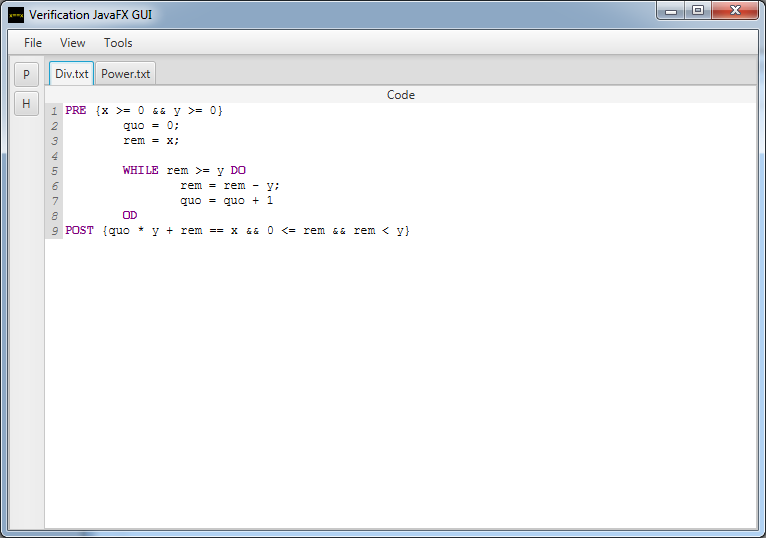
\includegraphics[width=\textwidth]{images/gui_main.png}
	
	\caption{Main window}
	\label{fig:gui_main}
\end{figure}

\begin{figure}
	\centering
	
	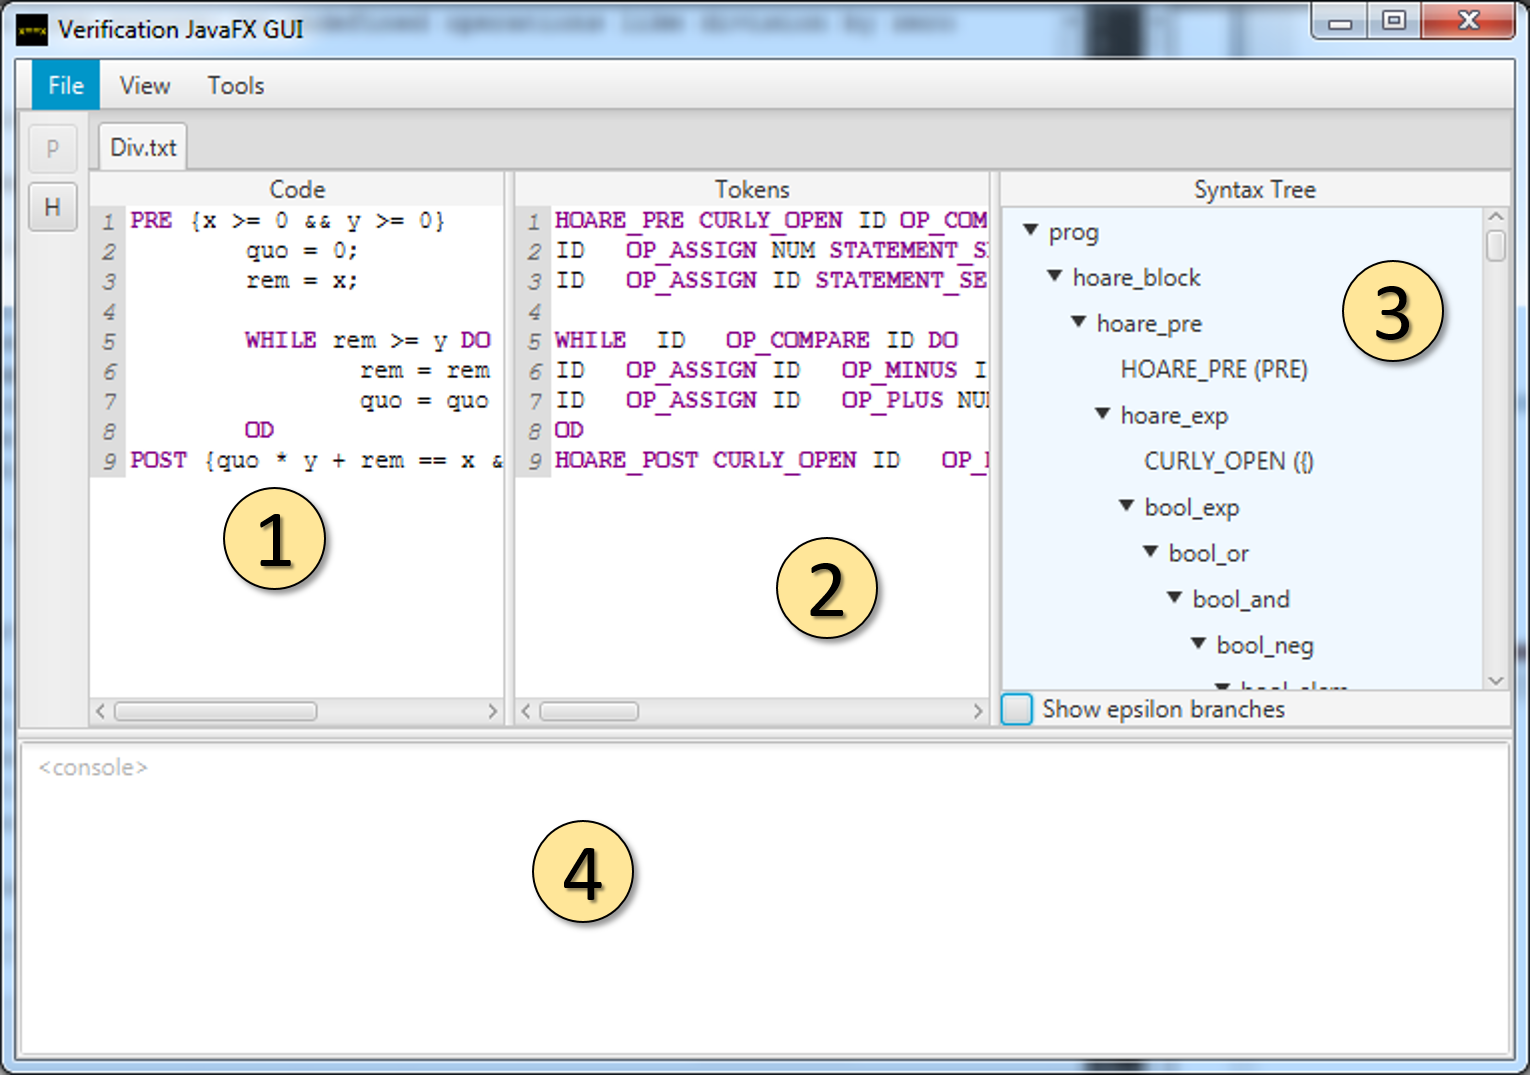
\includegraphics[width=\textwidth]{images/gui_tokens_syntaxTree.png}
	
	\caption{Views}
	\label{fig:gui_views}
\end{figure}

\section{Grammar, Lexer, parser}

A grammar hosts terminals and non terminal symbols, which come with their respective rules. Terminals are defined by lexer rules. Those are either regular expressions or fixed terms especially used for keywords. Parser rules for non terminals consist of an ordered list of a combination of non terminals and terminals. Therefore, \textclass{Symbol} was chosen as an abstract class generalizing \textclass{Terminal} and \textclass{NonTerminal}. The relationship is depicted in \figref{fig:class_grammar} and an example for the \textnonterminal{exp} grammar is found in \lstref{lst:grammar_exp}.

\begin{figure}[!h]
	\centering

	\begin{scaletikzpicturetowidth}{\textwidth}
\begin{tikzpicture}[scale=\tikzscale]
	\begin{umlpackage}{Grammar}
		\umlclass[x=11, y=0, type=abstract]{Symbol}{ String : key }{}
		
		\umlclass[x=6, y=-3]{ParserRule}{ symbols : List<Symbol>  }{}
		\umlclass[x=8,y=-6]{NonTerminal}{ rules : Set<ParserRule>  }{}
		\umlclass[x=14,y=-6]{Terminal}{ rules : Set<LexerRule> }{}
		\umlclass[x=18, y=-3]{LexerRule}{ exp : String \\ isRegex : bool }{}
		
		\umlclass[x=11, y=-10]{Grammar}{ nonTerminals : Set<NonTerminal> \\ terminals : Set<Terminal> }{}
		
		\umlinherit[geometry=-|]{Terminal}{Symbol}
		\umlinherit[geometry=-|]{NonTerminal}{Symbol}
		
		\umlcompo[geometry=-|, mult=*, pos=1.7]{Grammar}{NonTerminal}
		\umlcompo[geometry=-|, mult=*, pos=1.7]{Grammar}{Terminal}
		\umlcompo[geometry=-|, mult=*, pos=1.7]{Terminal}{LexerRule}
		\umlcompo[geometry=-|, mult=*, pos=1.7]{NonTerminal}{ParserRule}

		\umlaggreg[pos=0.8, mult=*]{ParserRule}{Symbol}
	\end{umlpackage}
\end{tikzpicture}
\end{scaletikzpicturetowidth}

	\caption{grammar-related class diagram}
	\label{fig:class_grammar}
\end{figure}

\lstinputlisting[caption={Implementation of \textnonterminal{exp} grammar (Java)},label={lst:grammar_exp}]{lst/exp_grammar.java}

The \textclass{Grammar} class can be extended, e.g. \textclass{ExpGrammar} is inherited by \textclass{WhileGrammar} (the grammar that describes while programs). This modularization approach concedes further flexibility when converting between string and syntax tree. An instance of \textclass{Grammar} both is used by the lexer and the parser. The \textclass{Lexer} class splits a string into a stream of tokens and the \textclass{Parser} class transforms the tokens into a syntax tree. \textclass{Token} is an aggregate of \textclass{Terminal} and contains additional details like the position it occupies relating to the input string. That information can be used for error reporting when checking the syntax or for other output arrangement.

The inner workings of the lexer can be looked at in \lstref{lst:lexer}. The method first removes comments and sanitizes the input from unnecessary line breaks. The current position is memorized and incorporated into the regular expression pattern. All of the terminals and rules are iterated over in order to find the longest match. Before doing that, the rules get sorted because the language for \textterminal{id} is infact a superset of most keywords like \textterminal{IF} or \textterminal{WHILE}. In that case, the keywords should be prioritized. If no match is found after trying everything, an exception with the current position will be thrown. Otherwise, the longest match will generate a new instance of \textclass{Token} and the lexer appends it to the output list. The pointer advances and the process is repeated until it transcends the end of the input string.

Using the terminals and non terminals along with the information about the parser rules, a grammar can construct a predictive parser table. This table makes a direct assignment between a pair of \textclass{NonTerminal} and \textclass{Terminal} and \textclass{ParserRule} and is used by the parser to select the next rule. The parsing algorithm is depicted in \lstref{lst:parser}. First the terminator symbol (\textterminal{\$}) is annexed to the token list and the iterator is pointed to the first token. Beginning with the designated starting rule of the grammar, the recursively invoked \textmethod{getNode} method is called. It is supposed to create a single node of the syntax tree (paying attention to the current non terminal and token) but triggers the construction of all children nodes in one fell swoop. The \textmethod{selectRule} method fetches the rule to pursue from the predictive parser table and will report an error if there is no entry. Then the symbols of the rule are gone over: If a symbol is a terminal, it will be compared against the current token, added as a child and the iterator will take a step to point to the next token. In case of the empty word, the child is a special \textemph{\straightepsilon{}} node. Lastly, non terminals amount to a child as well but call the \textmethod{getNode} method again to acquire their own respective children. Since the last case does not effectuate a change in the token iterator, the grammar is expected to indeed be a \textlang{} grammar as a different scenario would be prone to induce an infinite loop.

\begin{figure}[!h]
	\centering

	\begin{tikzpicture}
	\begin{umlpackage}{Parsing}			
		\umlclass[x=14,y=0]{Terminal}{ rules : Set<LexerRule> }{}
		\umlclass[x=14,y=-3]{Token}{ terminal : Terminal \\ int : line }{}
		
		\umlclass[x=5, y=0]{Grammar}{ nonTerminals : Set<NonTerminal> \\ terminals : Set<Terminal> }{}
		\umlclass[x=5, y=-4]{ParserTable}{ map : Map<Pair<\\ NonTerminal, Terminal>\\ , ParserRule> }{}

		\umlclass[x=5, y=-8]{Parser}{}{ parse(Grammar grammar,\\ List<Token>) : SyntaxTree }
		\umlclass[x=10, y=-11]{SyntaxTree}{}{}
		\umlclass[x=14, y=-8]{Lexer}{}{ tokenize(grammar: Grammar,\\ input : String) : List<Token> }
		
		\umldep[geometry=--, pos=1.7,stereo=create]{Lexer}{Token}
		\umldep[geometry=--, pos=1.7,stereo=use]{Parser}{ParserTable}
		\umldep[geometry=--, pos=1.7,stereo=use]{Parser}{Token}
		\umldep[geometry=|-, pos=1.7,stereo=create]{Parser}{SyntaxTree}
		\umlcompo[geometry=--, pos=1.7]{Grammar}{ParserTable}
		\umlaggreg[geometry=--, pos=1.7]{Token}{Terminal}
	\end{umlpackage}
\end{tikzpicture}

	\caption{parser-related class diagram}
	\label{fig:class_parser}
\end{figure}

\subsection{First, follow}

The algorithms for the concept of \textname{First} and \textname{Follow} were already outlined in \chref{Introduction of language}. Specific \textname{Java} implementations are provided in \lstref{lst:getFirst_abstract} and \lstref{lst:getFollow_abstract}. The predictive parser table is pieced together in \lstref{lst:parser_table};

\lstinputlisting[caption={Implementation of First (Java)},label={lst:getFirst_abstract}]{lst/getFirst_abstract.java}

\lstinputlisting[caption={Implementation of Follow (Java)},label={lst:getFollow_abstract}]{lst/getFollow_abstract.java}

\lstinputlisting[caption={Parser table (Java)},label={lst:parser_table}]{lst/parser_table.java}

\lstinputlisting[caption={Lexer (Java)},label={lst:parser_table}]{lst/lexer.java}

\lstinputlisting[caption={Parser (Java)},label={lst:parser}]{lst/parser.java}

\section{Hoare}

\section{Exception handling}

\section{GUI}

\subsection{Editor}
\subsection{Display of tokens/syntax tree}
\subsection{Syntax chart with Hoare decoration}

\chapter{Fazit}\label{ch:fazit}
\section{Summerization}
\section{Remaining problems}
\section{Extendabilities}

\cite{gate_compiler_design}

\bibliographystyle{alphaurl}
\nocite{*}
\bibliography{lib}

%START OF APPENDIX
\appendix

\chapter{First, Follow, Parser Table listings}\label{app:parser_table}

\lstinputlisting[label={lst:getFirst}]{lst/getFirst.java}
\newpage
\lstinputlisting[label={lst:getFollow}]{lst/getFollow.java}
\newpage
\lstinputlisting[label={lst:parser_table}]{lst/parser_table.java}

\chapter{Lexer, Parser listings}\label{app:lexer_parser}

\lstinputlisting[label={lst:lexer}]{lst/lexer.java}
\lstinputlisting[label={lst:parser}]{lst/parser.java}

\chapter{Hoare listing}\label{app:lexer_parser}

\lstinputlisting[label={lst:hoare}]{lst/hoare.java}

\chapter{Grammmar for while programs}\label{app:grammar_core}

\begin{grammarEx}
	<num> ::= [1-9][0-9]*
	\alt 0
	
	<id> ::= [a-zA-Z][a-zA-Z0-9]*
	
	<exp> ::= <factor> <exp'> 
	
	<exp'> ::= \lit{+} <factor> <exp'> 
	\alt \lit{-} <factor> <exp'> 
	\alt \straightepsilon{} 
	
	<factor> ::= <pow> <factor'> 
	
	<factor'> ::= \lit{*} <pow> <factor'> 
	\alt \lit{/} <pow> <factor'> 
	\alt \straightepsilon{} 
	
	<pow> ::= <factorial> <pow'> 
	
	<pow'> ::= \lit{\^{}} <pow> 
	\alt \straightepsilon{} 
	
	<factorial> ::= <exp\textunderscore elem> <factorial'> 
	
	<factorial'> ::= \lit{!} 
	\alt \straightepsilon{} 
	
	<exp\textunderscore elem> ::= \lit{id} 
	\alt \lit{num} 
	\alt \lit{(} <exp> \lit{)} 
	
	<bool\textunderscore exp> ::= <bool\textunderscore or> 
	
	<bool\textunderscore or> ::= <bool\textunderscore and> <bool\textunderscore or'> 
	
	<bool\textunderscore or'> ::= \lit{\textbar\textbar} <bool\textunderscore and> <bool\textunderscore or'> 
	\alt \straightepsilon{} 
	
	<bool\textunderscore and> ::= <bool\textunderscore neg> <bool\textunderscore and'> 
	
	<bool\textunderscore and'> ::= \lit{\&\&} <bool\textunderscore neg> <bool\textunderscore and'> 
	\alt \straightepsilon{} 
	
	<bool\textunderscore neg> ::= <bool\textunderscore elem> 
	\alt \lit{\textasciitilde{}} <bool\textunderscore elem> 
	
	<bool\textunderscore elem> ::= <exp> \lit{\textless{}} <exp> 
	\alt \lit{true} 
	\alt \lit{[} <bool\textunderscore exp> \lit{]} 
	
	<*prog> ::= <skip> <prog'> 
	\alt <assign> <prog'> 
	\alt <selection> <prog'> 
	\alt <while> <prog'> 
	
	<prog'> ::= \lit{;} <prog> 
	\alt \straightepsilon{} 
	
	<skip> ::= \lit{SKIP} 
	
	<assign> ::= \lit{id} \lit{=} <exp> 
	
	<selection> ::= \lit{IF} <bool\textunderscore exp> \lit{THEN} <prog> <selection\textunderscore else> \lit{FI} 
	
	<selection\textunderscore else> ::= \lit{ELSE} <prog> 
	\alt \straightepsilon{} 
	
	<while> ::= \lit{WHILE} <bool\textunderscore exp> \lit{DO} <prog> \lit{OD} 
\end{grammarEx}

\chapter{Grammar for Hoare-decorated while programs}\label{app:grammar_hoare}

\begin{grammarEx}
	<num> ::= [1-9][0-9]*
	\alt 0
	
	<id> ::= [a-zA-Z][a-zA-Z0-9]*
	
	<exp> ::= <factor> <exp'> 
	
	<exp'> ::= \lit{+} <factor> <exp'> 
	\alt \lit{-} <factor> <exp'> 
	\alt \straightepsilon{} 
	
	<factor> ::= <pow> <factor'> 
	
	<factor'> ::= \lit{*} <pow> <factor'> 
	\alt \lit{/} <pow> <factor'> 
	\alt \straightepsilon{} 
	
	<pow> ::= <factorial> <pow'> 
	
	<pow'> ::= \lit{\^{}} <pow> 
	\alt \straightepsilon{} 
	
	<factorial> ::= <exp\textunderscore elem> <factorial'> 
	
	<factorial'> ::= \lit{!} 
	\alt \straightepsilon{} 
	
	<exp\textunderscore elem> ::= \lit{id} 
	\alt \lit{num} 
	\alt \lit{(} <exp> \lit{)} 
	
	<bool\textunderscore exp> ::= <bool\textunderscore or> 
	
	<bool\textunderscore or> ::= <bool\textunderscore and> <bool\textunderscore or'> 
	
	<bool\textunderscore or'> ::= \lit{\textbar\textbar} <bool\textunderscore and> <bool\textunderscore or'> 
	\alt \straightepsilon{} 
	
	<bool\textunderscore and> ::= <bool\textunderscore neg> <bool\textunderscore and'> 
	
	<bool\textunderscore and'> ::= \lit{\&\&} <bool\textunderscore neg> <bool\textunderscore and'> 
	\alt \straightepsilon{} 
	
	<bool\textunderscore neg> ::= <bool\textunderscore elem> 
	\alt \lit{\textasciitilde{}} <bool\textunderscore elem> 
	
	<bool\textunderscore elem> ::= <exp> \lit{\textless{}} <exp> 
	\alt \lit{true} 
	\alt \lit{[} <bool\textunderscore exp> \lit{]} 
	
	<*prog> ::= <skip> <prog'> 
	\alt <assign> <prog'> 
	\alt <selection> <prog'> 
	\alt <while> <prog'> 
	\alt <hoare\textunderscore block> <prog'> 
	
	<prog'> ::= \lit{;} <prog> 
	\alt \straightepsilon{} 
	
	<skip> ::= \lit{SKIP} 
	
	<assign> ::= \lit{id} \lit{=} <exp> 
	
	<selection> ::= \lit{IF} <bool\textunderscore exp> \lit{THEN} <prog> <selection\textunderscore else> \lit{FI} 
	
	<selection\textunderscore else> ::= \lit{ELSE} <prog> 
	\alt \straightepsilon{} 
	
	<while> ::= \lit{WHILE} <bool\textunderscore exp> \lit{DO} <prog> \lit{OD} 
	
	<hoare\textunderscore exp> ::= \lit{\{} <bool\textunderscore exp> \lit{\}} 
	
	<hoare\textunderscore pre> ::= \lit{PRE} <hoare\textunderscore exp> 
	
	<hoare\textunderscore post> ::= \lit{POST} <hoare\textunderscore exp> 
	
	<hoare\textunderscore block> ::= <hoare\textunderscore pre> <prog> <hoare\textunderscore post> 
\end{grammarEx}

\clearpage
\phantomsection
\clearpage
\phantomsection

\section*{{\huge{}Declaration of Originality}}

I hereby confirm that I have written the accompanying thesis by myself, without contributions from any sources other than those cited in the text and acknowledgements.
This applies also to all graphics, drawings, maps and images included in the thesis.

\vspace{2cm}

\begin{center}
	\begin{tabular}{@{}p{5cm}@{}p{2cm}@{}p{5cm}}
		Merseburg, \today & &  \\
		\dotfill & & \dotfill \\
		\emph{Place and date} & & \emph{Signature} \\
	\end{tabular}
	\par
\end{center}

\newpage

\section*{{\huge{}Dedication and Acknowledgements}}

\end{document}

%START OF DUMP
questions:
-cite ref article/direct
-grammar ref
-ref online/book/both?

verschiedene semantiken
operationell: schrittweise ausführung
werte der variablen, restprogramm kennen
untersuchung output oder zwischenergebnisse
Halteproblem

zustand: abbildung z: var teilmenge var(prog) -> wert(x1) v wert(x2) ... wert(xm)
+help vars
z(xi) element wert(xi) i=1,...,m
zust(prog) menge aller states

auswertung semantik
Sem(x,z)=z(x)

\cite{motivation_science}

%\printbibliography

modern languages no null objects, frequent source of error (NullPointerException)
ProofCarryingCode, code devoid of proofs

correctness important, program has to fulfill specifications/properties

correct results
termination
no runtime errors

operational reasoning usual in programmer's everyday life but bad
denotational reasoning
fixed point semantics

here: axiomatic reasoning, predicate logic to specify properties
assertions

axiomatic approach limits:
verification, not development
only input/output characteristics, not of finite/infinite operations
no fairness assumptions

%temporal logic:
%liveness properties
%fairness

classes of programs
while program
%fine-tuned verification methods for each class

theory of computability general verification undecidable, finite-state systems -> possible
model checking -> program is model of specification?
program analysis -> similar to model checking, dynamic behavior analyzed, has variable value at control point?

%deductive verification automates axiomatic approach
%ApplicativeCommonLisp
%Isabelle/HOL



usual desired features of sequential programs:

partial correctness: if the algorithm returns a result (terminates),
it is correct in reference to the statement of the problem. The termination
is not guaranteed.

termination: the algorithm terminates for all designated inputs, else
the algorithm is said to diverge

no run time errors: no undefined operations like division by zero
occur

example: different sorting algorithms

mathematical logic

what is correctness

the disadvantages of the axiomatic approach are that those rules are
only suited for the verification, not for the development of a program,
only the behavior in reference to input/output, not considering finite/infinite
executions (operating system), fairness is ignored

proof system for each class of programs


%\chapter{Excursions}\label{ch:Excursions}
%
%\section{Shape analysis}
%\section{Model checking}
%automata, petri nets
%\section{Alternative logics}
%linear temporal logic (LTL), timed computation tree logic (TCTL)

what is not covered, parallelism, deadlock, inference, fairness